\documentclass{beamer}
\usetheme{ttuStatsCamp}
\usefonttheme{serif}
\usepackage[T1]{fontenc}
\usepackage[utf8]{inputenc}
\usepackage{url}
\usepackage{graphicx}
\usepackage{setspace}
\usepackage[natbibapa]{apacite}
\usepackage{color}
\usepackage{amsmath}
\usepackage{amsfonts}
\usepackage{Sweavel}
\usepackage{listings}
\usepackage{fancybox}

\def\Sweavesize{\scriptsize}
\def\Rcolor{\color{black}}
%\def\Routcolor{\color{red}}
\def\Rcommentcolor{\color{violet}}
\def\Rbackground{\color[gray]{0.85}}
\def\Routbackground{\color[gray]{0.85}}

\lstset{tabsize=2, breaklines=true, style=Rstyle}



\newcommand{\red}[0]{\textcolor{red}}
\newcommand{\green}[0]{\textcolor{green}}
\newcommand{\blue}[0]{\textcolor{blue}}
\newcommand{\comment}[1]{}
\newcommand{\va}[0]{\vspace{12pt}}
\newcommand{\vb}[0]{\vspace{6pt}}
\newcommand{\vc}[0]{\vspace{3pt}}
\newcommand{\vx}[1]{\vspace{#1pt}}

\title[Lecture 10]{Lecture 10: Conditional Process Analysis}

\author{Kyle M. Lang}

\institute[TTU IMMAP]{
  Institute for Measurement, Methodology, Analysis \& Policy\\
  Texas Tech University\\
  Lubbock, TX
}

\date{2016 Stats Camp}

\setbeamertemplate{frametitle continuation}{}

\begin{document}

\setkeys{Gin}{width=\textwidth}

\input{sweaveFiles/-001}


\begin{frame}[plain]
  
  \titlepage
  
\end{frame}


\begin{frame}{Outline}

  \begin{itemize}
  \item Conceptual introduction to conditional process analysis
    \va
  \item Define conditional direct and indirect effects
    \va
  \item Examples of some basic conditional process models
    \va
  \item Run through some basic examples of conditional process models
  \end{itemize}
  
\end{frame}



\begin{frame}{Starting Point}
  
  So far, we've been discussing mediation and moderation as
  independent hypotheses.  
  \va
  \begin{itemize}
    \item With mediation, we're interested in describing the chain of
      events by which $X$ influences $Y$.
      \vb
      \begin{itemize}
      \item We want to model the process by which $X$ affects $Y$.
        \vc
      \item We're asking questions about \emph{how} $X$ impacts $Y$.
      \end{itemize}
      \vb
    \item With moderation, we're interested in discovering how the
      relation between $X$ and $Y$ changes as a function of some
      moderating variable (or set of moderating variables).  
      \vb
      \begin{itemize}
      \item We want to know at what levels of the moderator is the $X
        \rightarrow Y$ relation statistically significant.
        \vc
      \item We're asking questions about \emph{when} $X$ affects $Y$.
      \end{itemize}
  \end{itemize}
  
\end{frame}



\begin{frame}{Conditional Process Analysis}
  
  We can combine the \emph{how}-type questions answer by mediation
  models and the \emph{when}-type questions answered by moderation
  analysis via \emph{conditional process analysis}.
  \va
  \begin{itemize}
    \item With conditional process analysis, we're interested in
      assessing how an indirect effect (i.e., a process) changes as a
      function of some set of moderating variables (i.e., is
      conditional on those moderators).
      \vb
    \item We want to estimate \emph{conditional indirect (direct)
      effects}.  
      \vb
    \item This type of model is often called \emph{moderated
      mediation}.
  \end{itemize}
  
\end{frame}


\begin{frame}{Conditional Process Analysis}
  
  We can also ask questions about how the effect of an interaction
  term is transmitted through a mediator to the focal outcome.
  \va
  \begin{itemize}
    \item This type of model is called \emph{mediated moderation}.
      \vb
    \item It turns out that mediated moderation is mathematically
      equivalent to moderated mediation.
      \vb
    \item Mediated moderation is, nearly always, impossible to
      interpret (more on that later).
  \end{itemize}
  
\end{frame}



\begin{frame}{Simplest Example}
  
  The simplest example of a conditional process model includes only
  the direct effect as conditional:
  \vb
  \begin{figure}
    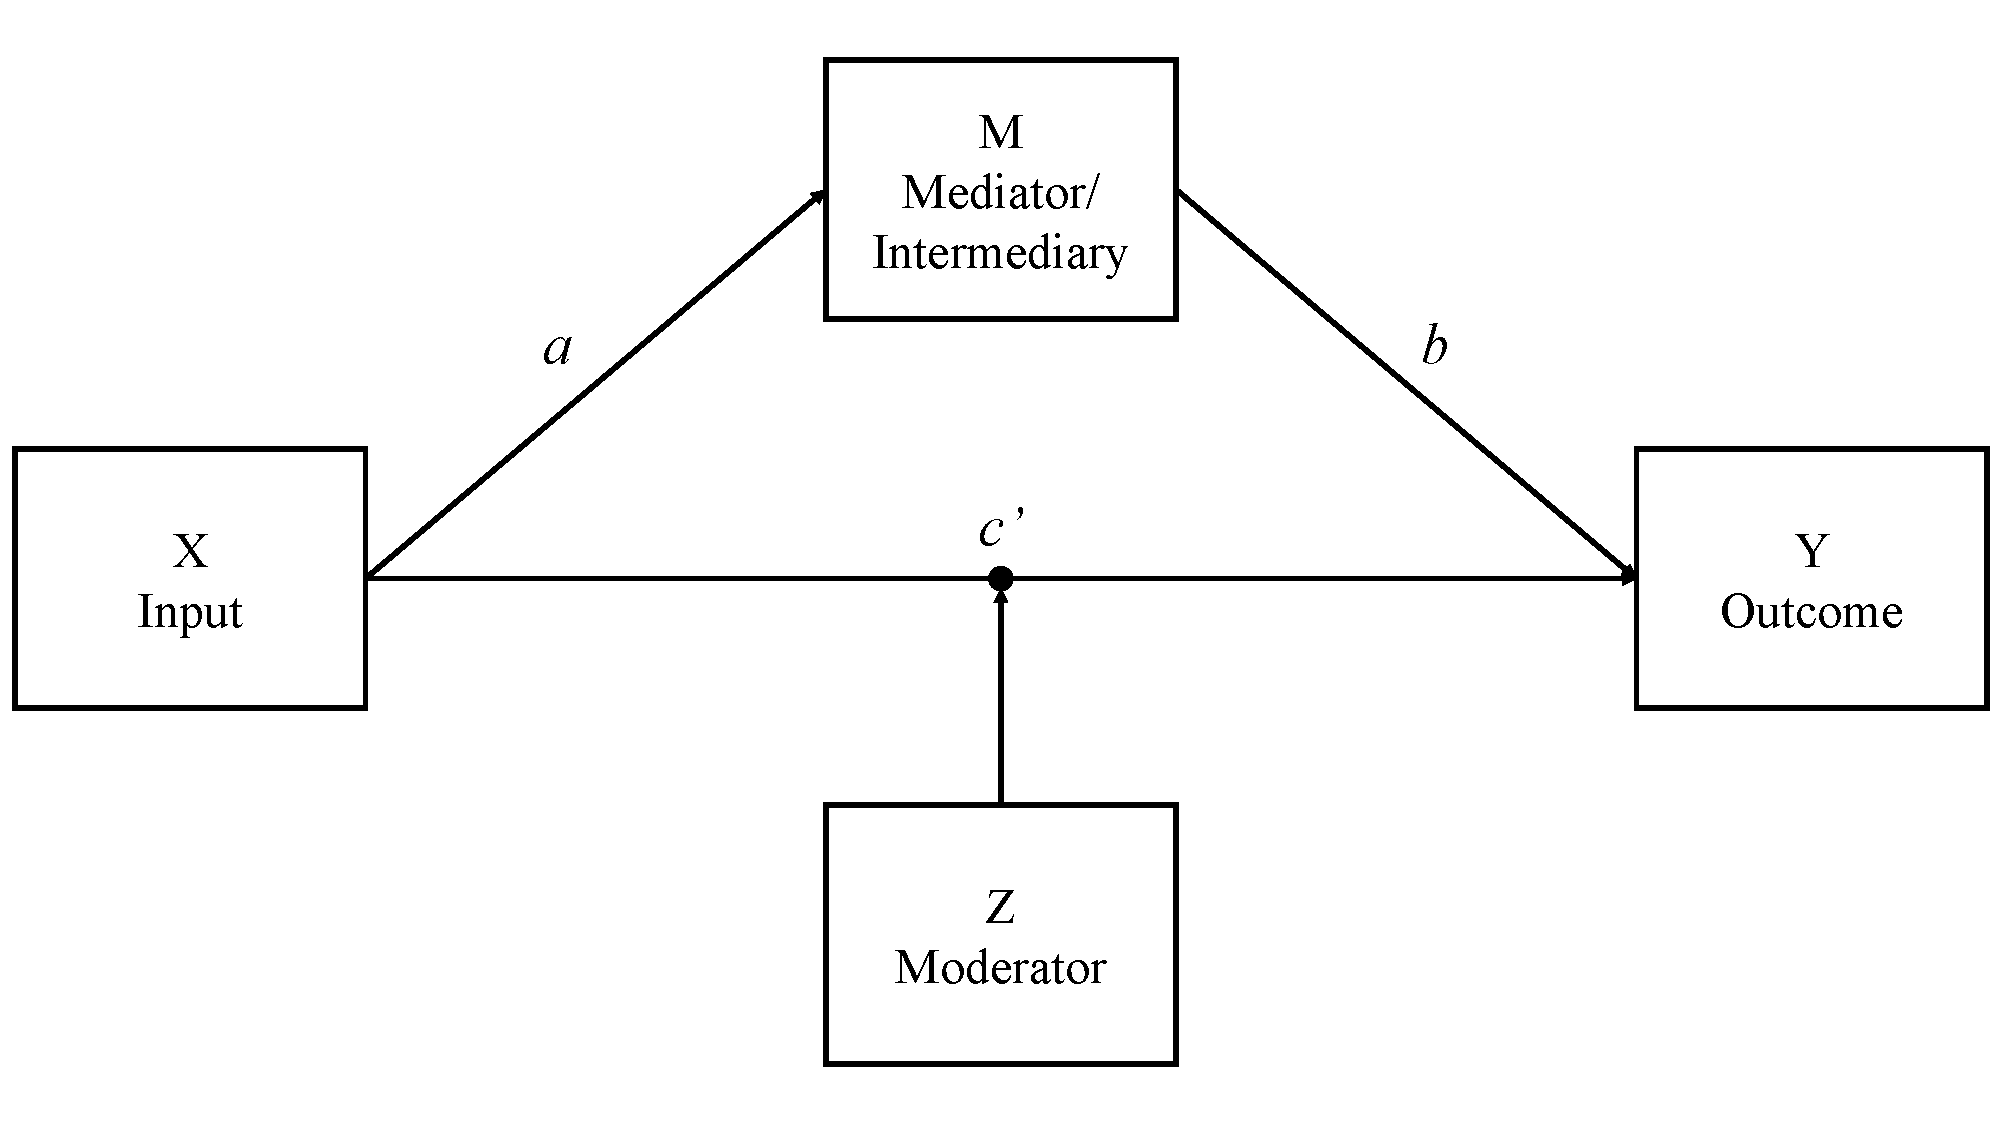
\includegraphics[width=0.95\textwidth]{figures/modCwithZConceptual.pdf}
  \end{figure}
  
\end{frame}


\begin{frame}{Simplest Example}
  
  The preceding conceptual diagram corresponds to the following
  analytic diagram: 
  \vb
  \begin{figure}
    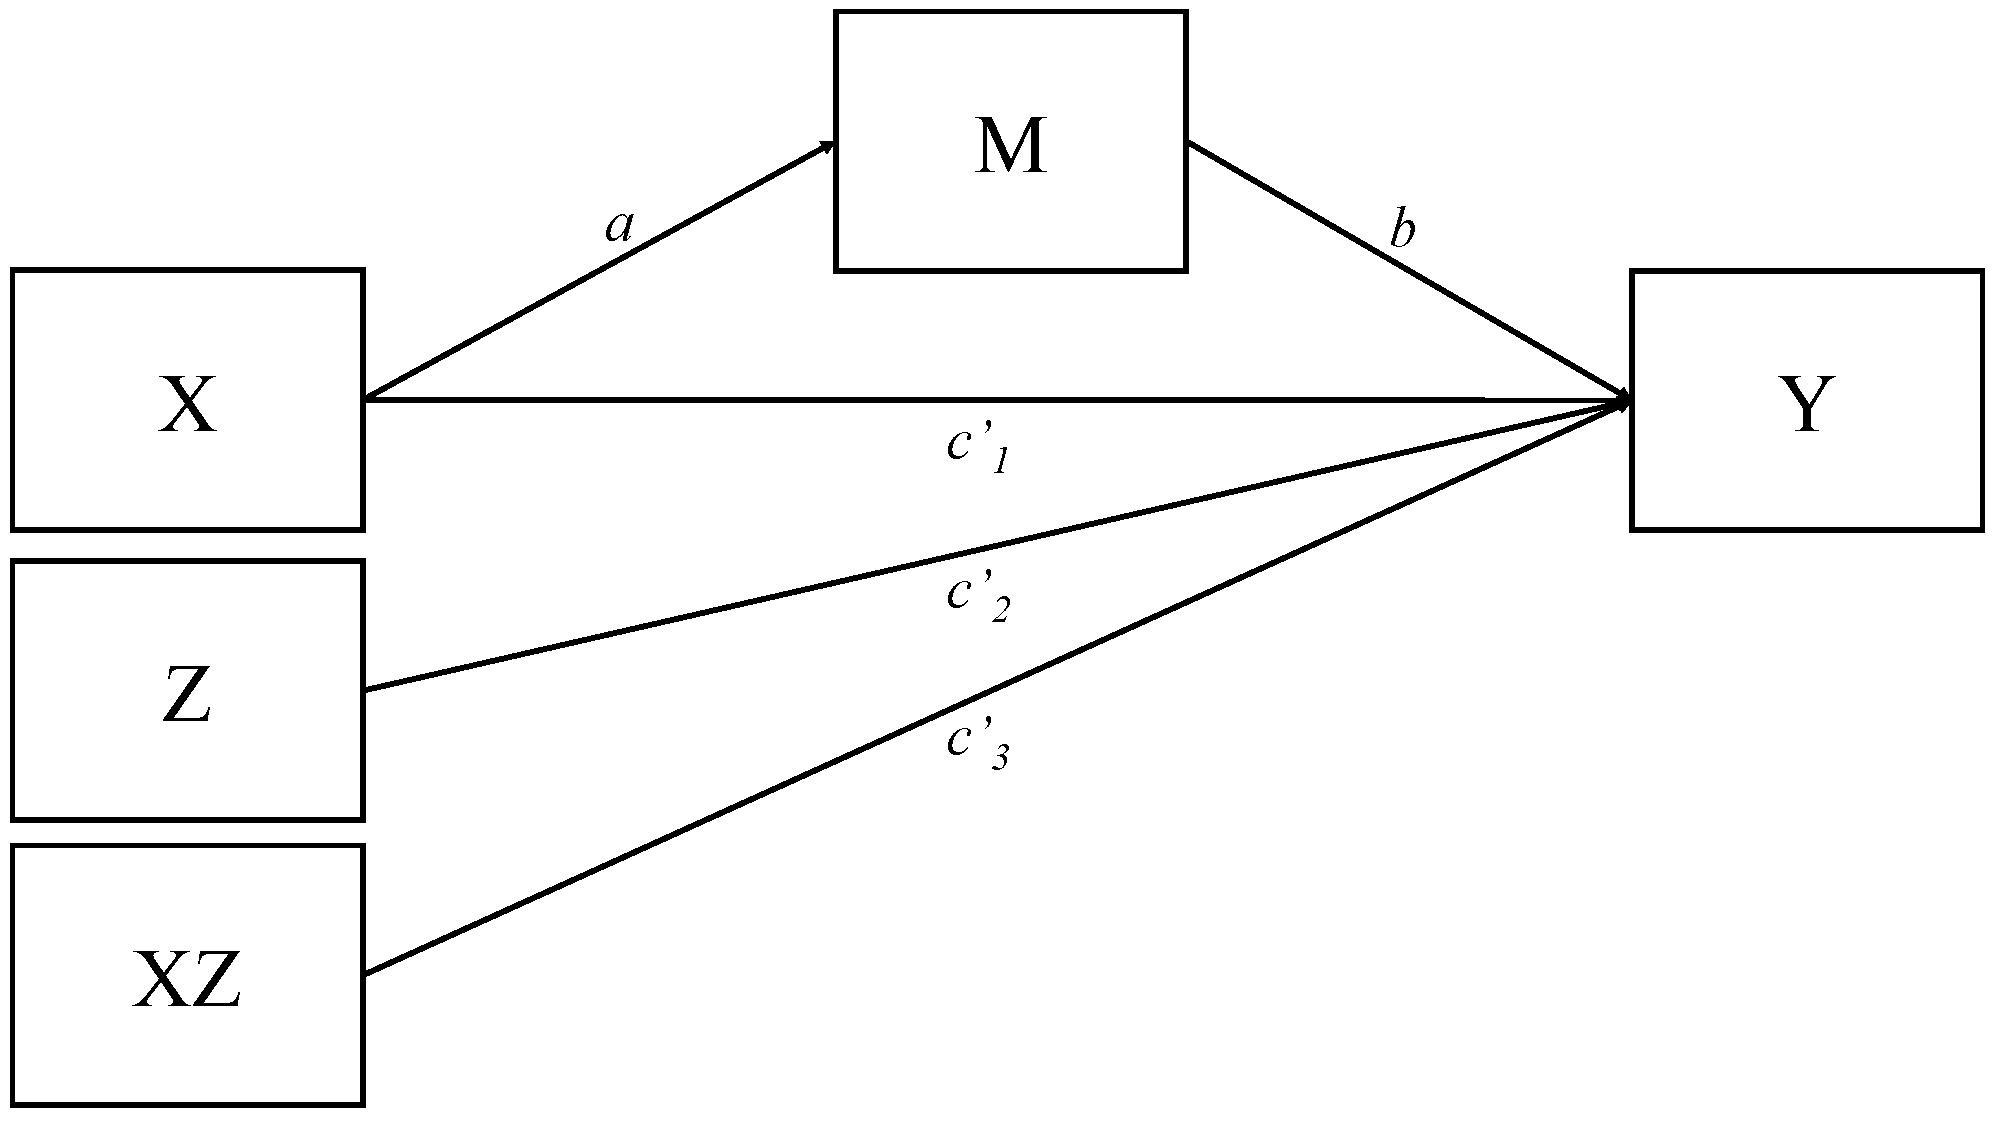
\includegraphics[width=0.95\textwidth]{figures/modCwithZAnalytic.pdf}
  \end{figure}
  
\end{frame}



\begin{frame}{Simplest Example}
  
  This analytic diagram implies the following equations:
  \begin{align}
    Y &= i_1 + bM + c_1'X + c_2'Z + c_3'XZ + e_Y \label{simpleEq1}\\
    M &= i_2 + aX + e_M
  \end{align}
  \pause
  In this simple case, the indirect effect is not conditional, so it
  is defined as before:
  \begin{align*}
    IE = ab
  \end{align*}
  \pause
  The direct effect, on the other hand, must be interpreted as
  conditional on $Z$.\\ 
  \va 
  \pause
  We can rearrange Equation \ref{simpleEq1} to get:
  \begin{align*}
    Y = i_1 + bM + c_2'Z + \left( c_1' + c_3'Z \right)X + e_Y
  \end{align*}
  The conditional direct effect is the simple slope linking $X$ to $Y$:
  \begin{align*}
    DE = c_1' + c_3'Z
  \end{align*}
  
\end{frame}



\begin{frame}{Another Example}
  
  A somewhat more interesting example of a conditional process model
  includes a conditional indirect effect induced by moderation of the
  $a$ path: 
  \vb
  \begin{figure}
    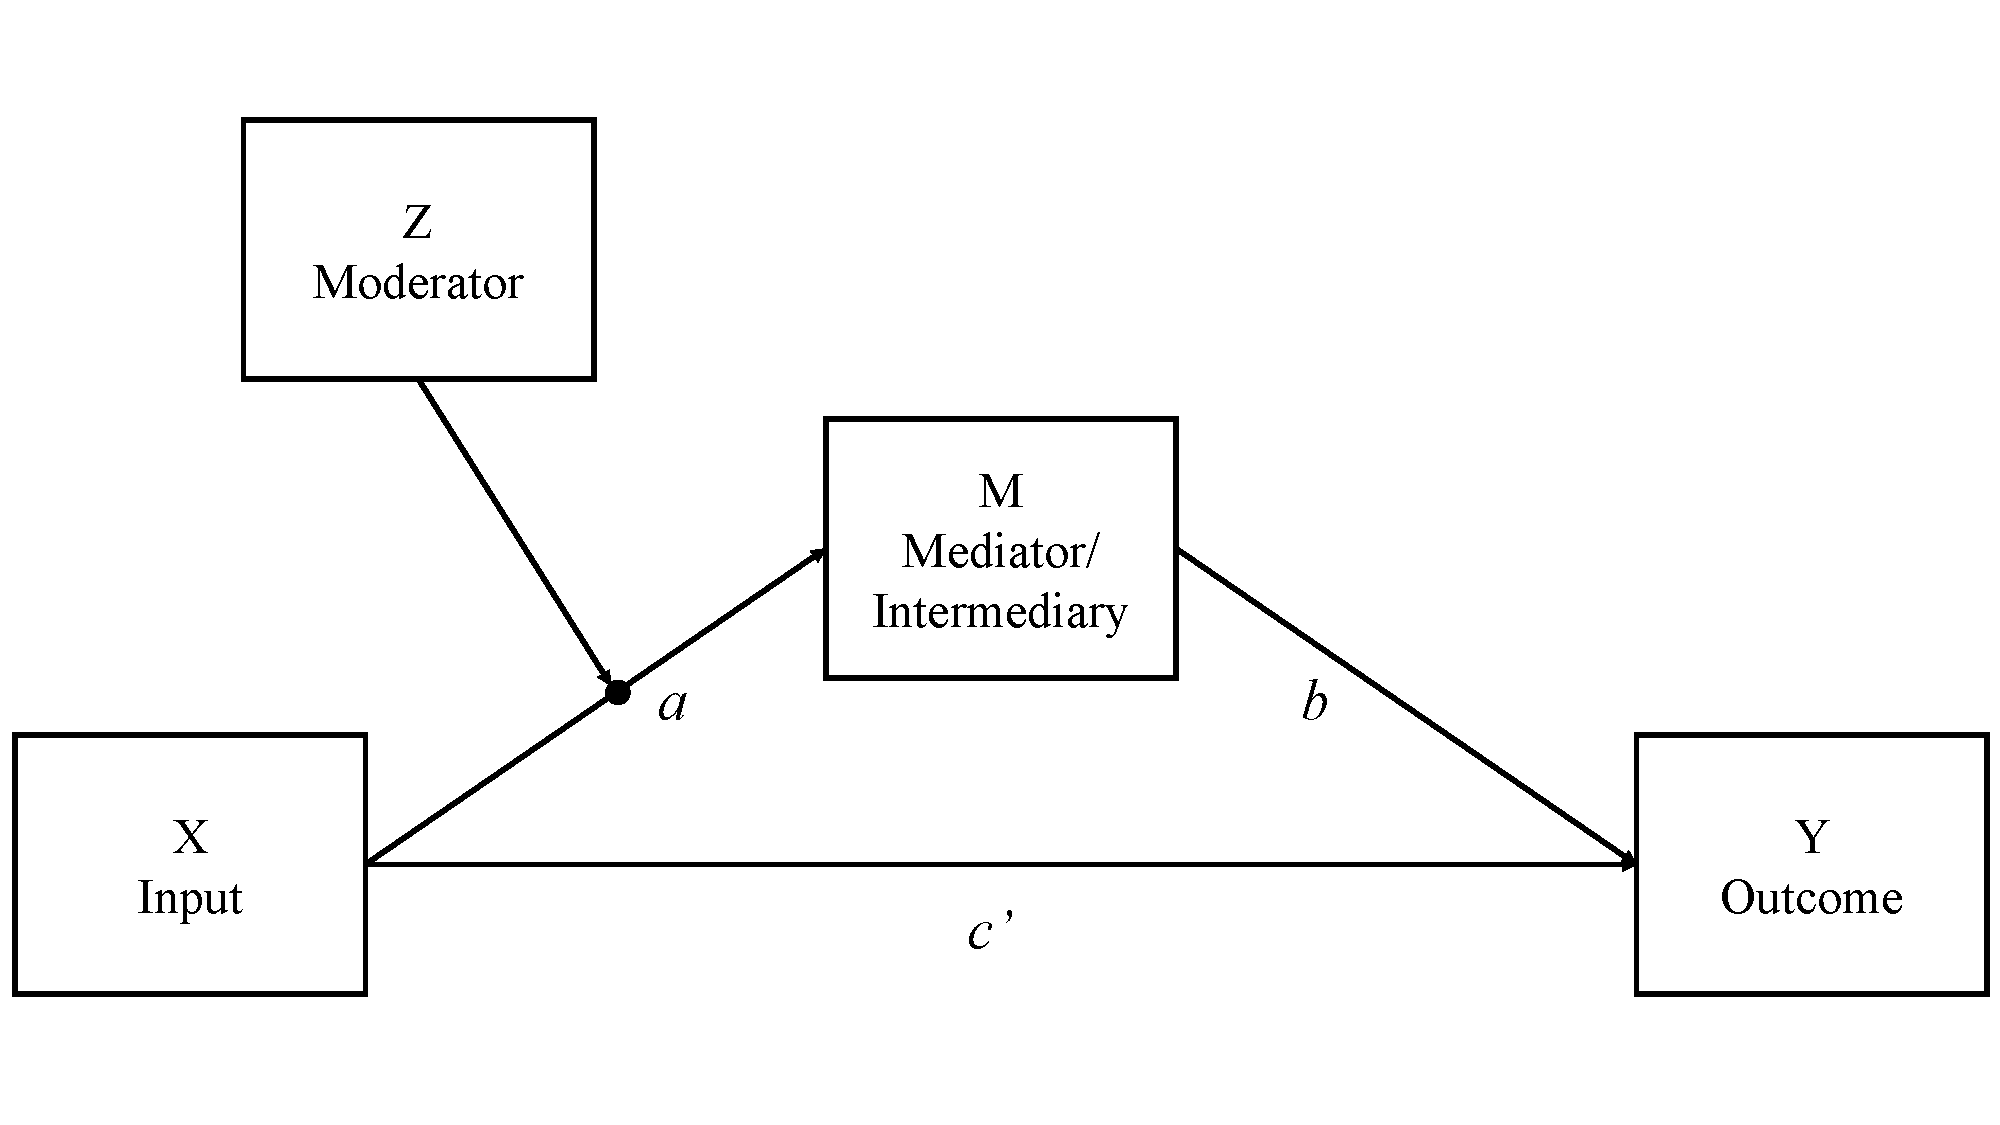
\includegraphics[width=0.95\textwidth]{figures/modAwithZConceptual.pdf}
  \end{figure}
  
\end{frame}



\begin{frame}{Another Example}
  
  The preceding conceptual diagram corresponds to the following
  analytic diagram: 
  \vb
  \begin{figure}
    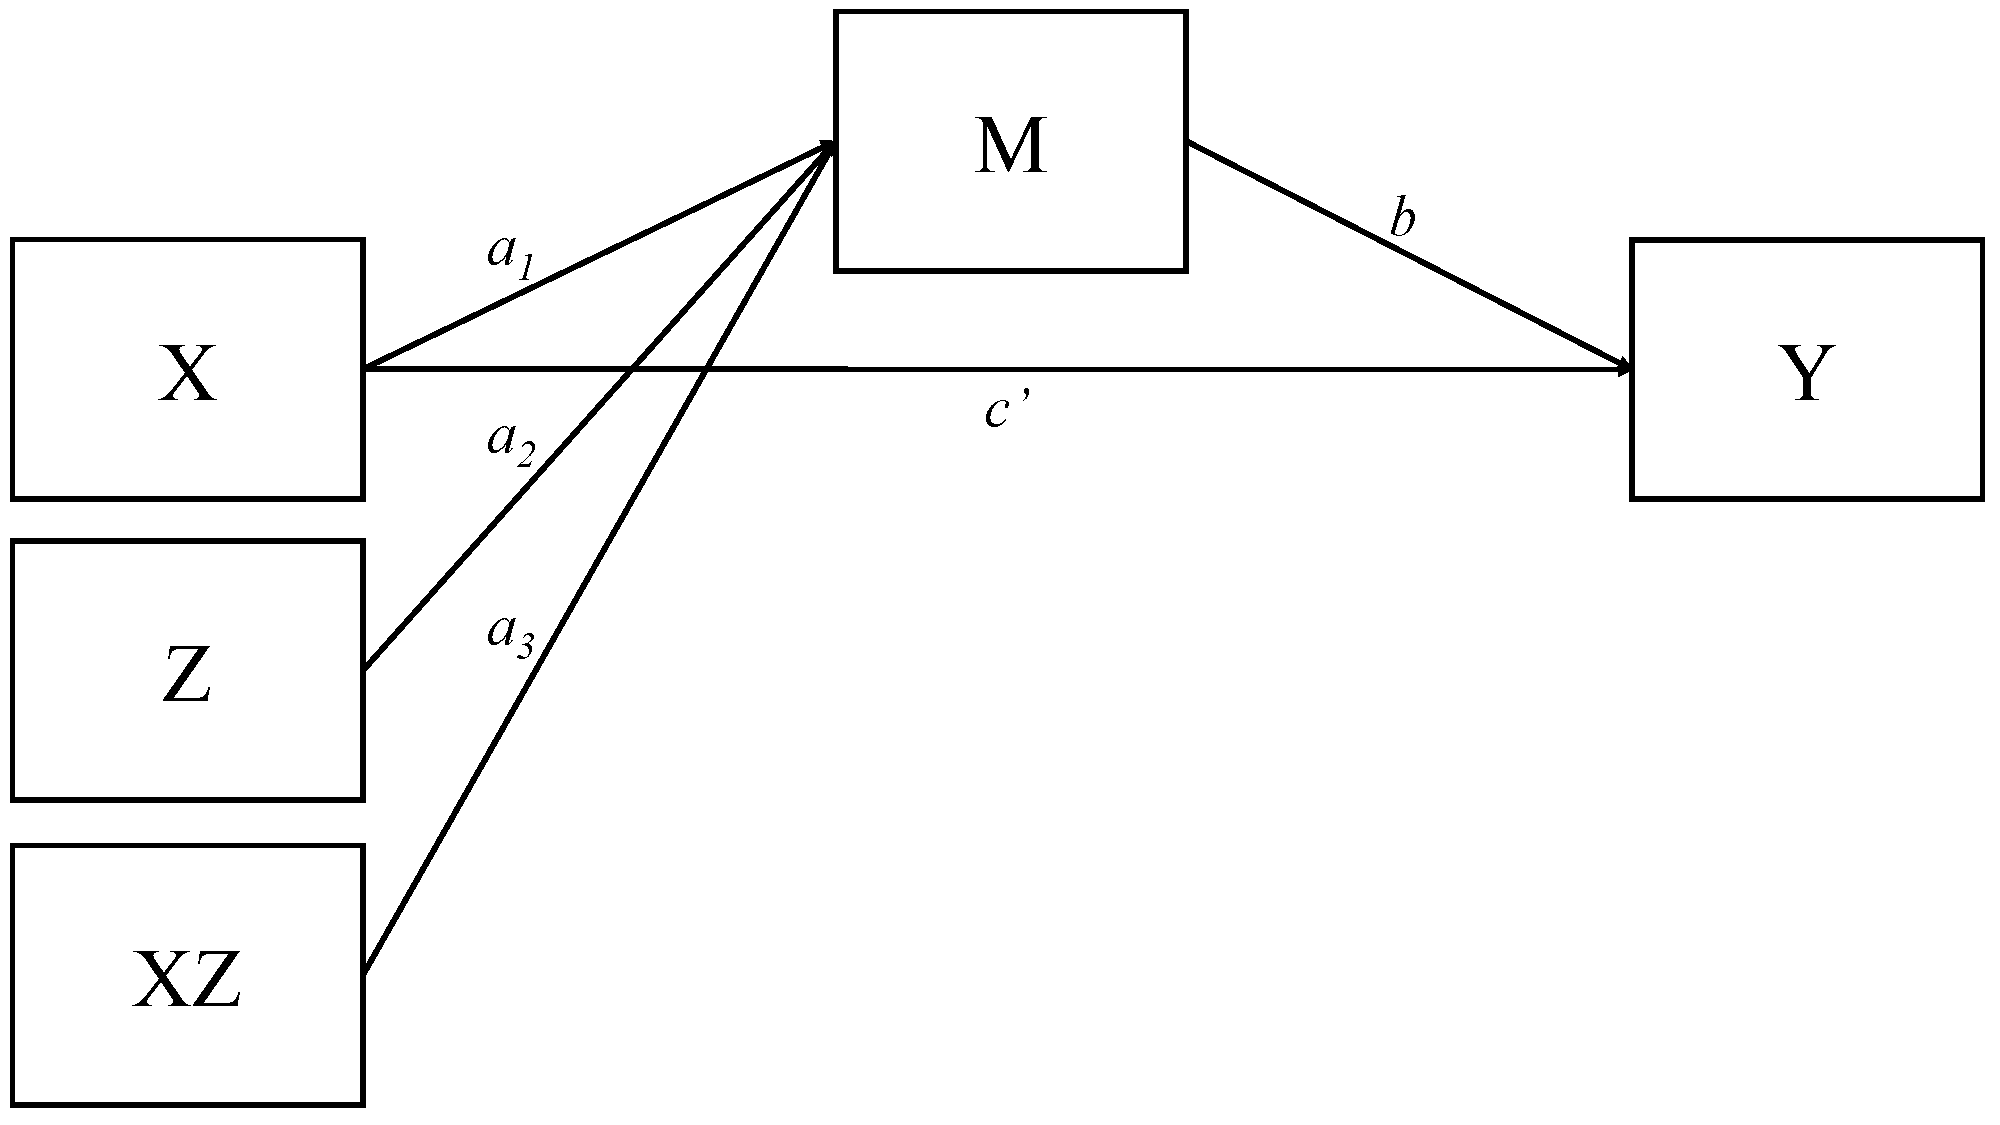
\includegraphics[width=0.95\textwidth]{figures/modAwithZAnalytic.pdf}
  \end{figure}
  
\end{frame}



\begin{frame}{Another Example}
  
  This analytic diagram implies the following equations:
  \begin{align}
    Y &= i_1 + bM + c'X + e_Y\\
    M &= i_2 + a_1X + a_2Z + a_3XZ + e_M \label{eq2}
  \end{align}
  \pause
  In this case, the direct effect is now unconditional, so it
  is defined as in simple mediation analysis:
  \begin{align*}
    DE = c'
  \end{align*}
  \pause 
  Now, the indirect effect must be interpreted as conditional
  on $Z$ due to the $a$ path being moderated by $Z$.\\ 
  \va 
  \pause 
  We can rearrange Equation \ref{eq2} to get:
  \begin{align*}
    M = i_2 + a_2Z + \left( a_1 + a_3Z \right)X + e_M
  \end{align*}
  The conditional indirect effect is now defined by the following
  product:
  \begin{align*}
    IE = \left(a_1 + a_3Z \right) b
  \end{align*}
  
\end{frame}



\begin{frame}{Another Example}
  
  The conditional indirect effect can also be induced by moderation of
  the $b$ path: 
  \vb
  \begin{figure}
    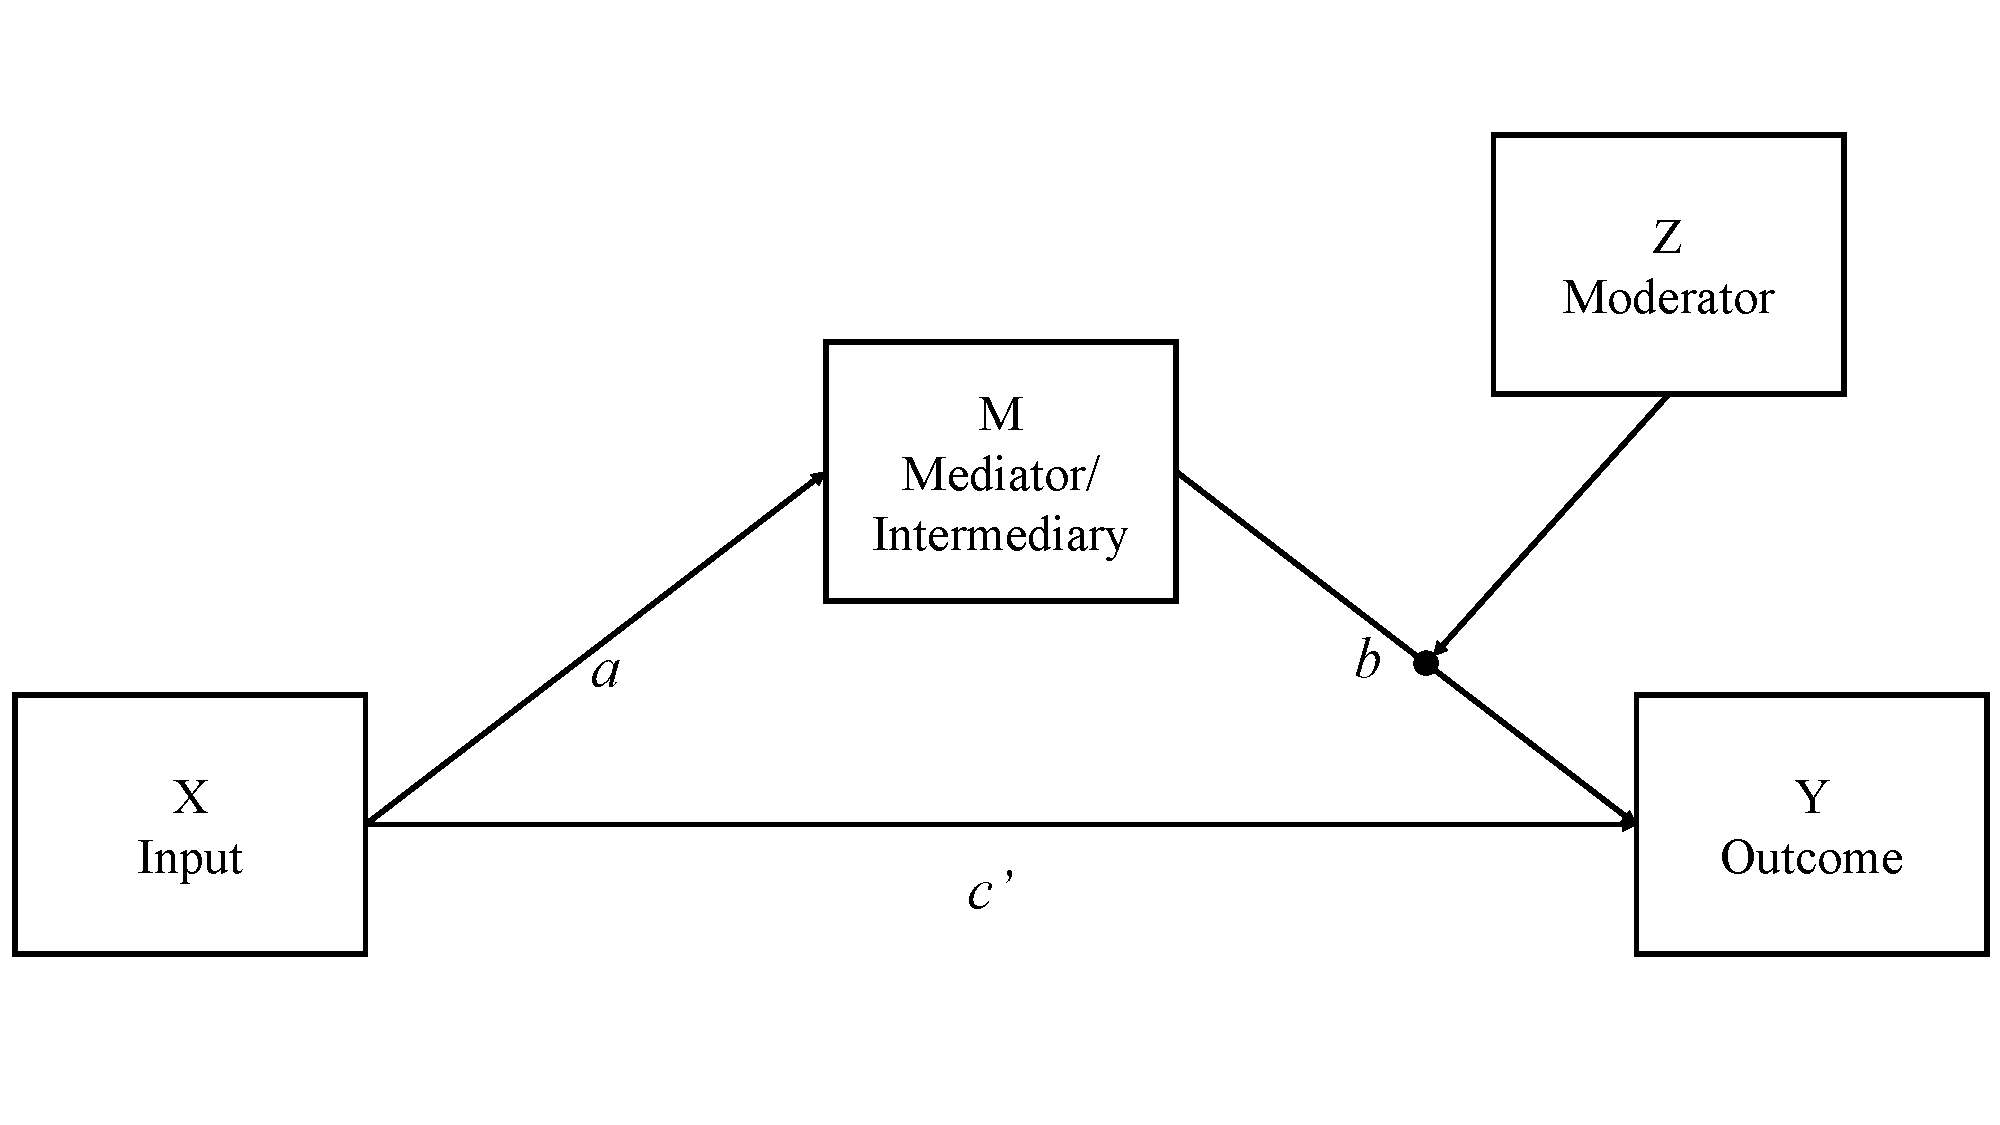
\includegraphics[width=0.95\textwidth]{figures/modBwithZConceptual.pdf}
  \end{figure}
  
\end{frame}



\begin{frame}{Another Example}
  
  The preceding conceptual diagram corresponds to the following
  analytic diagram: 
  \vb
  \begin{figure}
    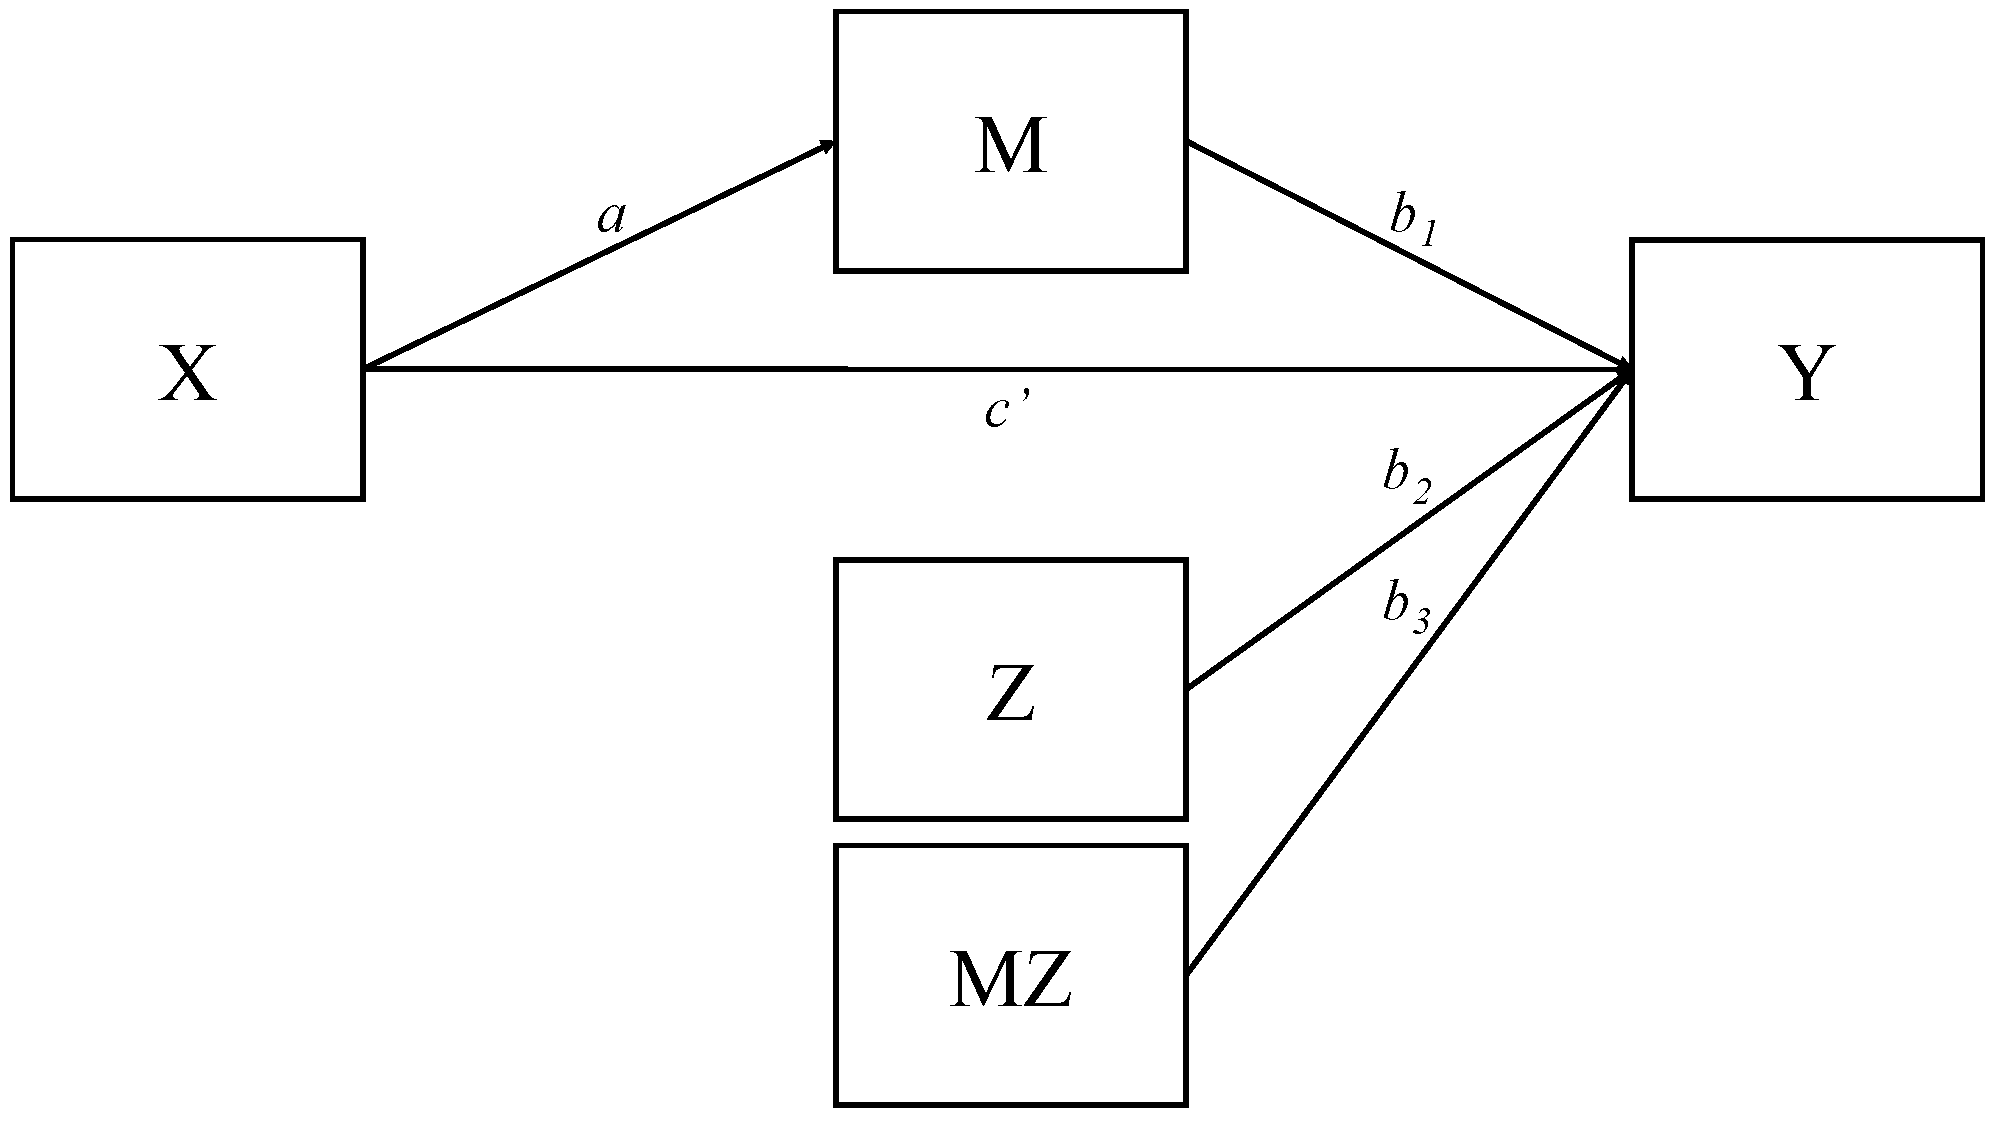
\includegraphics[width=0.95\textwidth]{figures/modBwithZAnalytic.pdf}
  \end{figure}
  
\end{frame}



\begin{frame}{Another Example}
  
  This analytic diagram implies the following equations:
  \begin{align}
    Y &= i_1 + c'X + b_1M + b_2Z + b_3MZ + e_Y \label{eq3}\\
    M &= i_2 + aX + e_M
  \end{align}
  \pause
  As above, the direct effect is unconditional:
  \begin{align*}
    DE = c'
  \end{align*}
  \pause 
  Again, the indirect effect is conditional on $Z$ due to the
  $b$ path being moderated by $Z$.\\ 
  \va 
  \pause 
  We can rearrange Equation \ref{eq3} to get:
  \begin{align*}
    Y = i_1 + b_2Z + \left( b_1 + b_3Z \right)M + e_Y
  \end{align*}
  So, the conditional indirect effect is defined by the following
  product:
  \begin{align*}
    IE = a \left(b_1 + b_3Z \right)
  \end{align*}
  
\end{frame}



\begin{frame}{Another Example}
  
  Maybe, we have a conditional indirect effect because $Z$ moderates
  both the $a$ and $b$ paths: 
  \vb
  \begin{figure}
    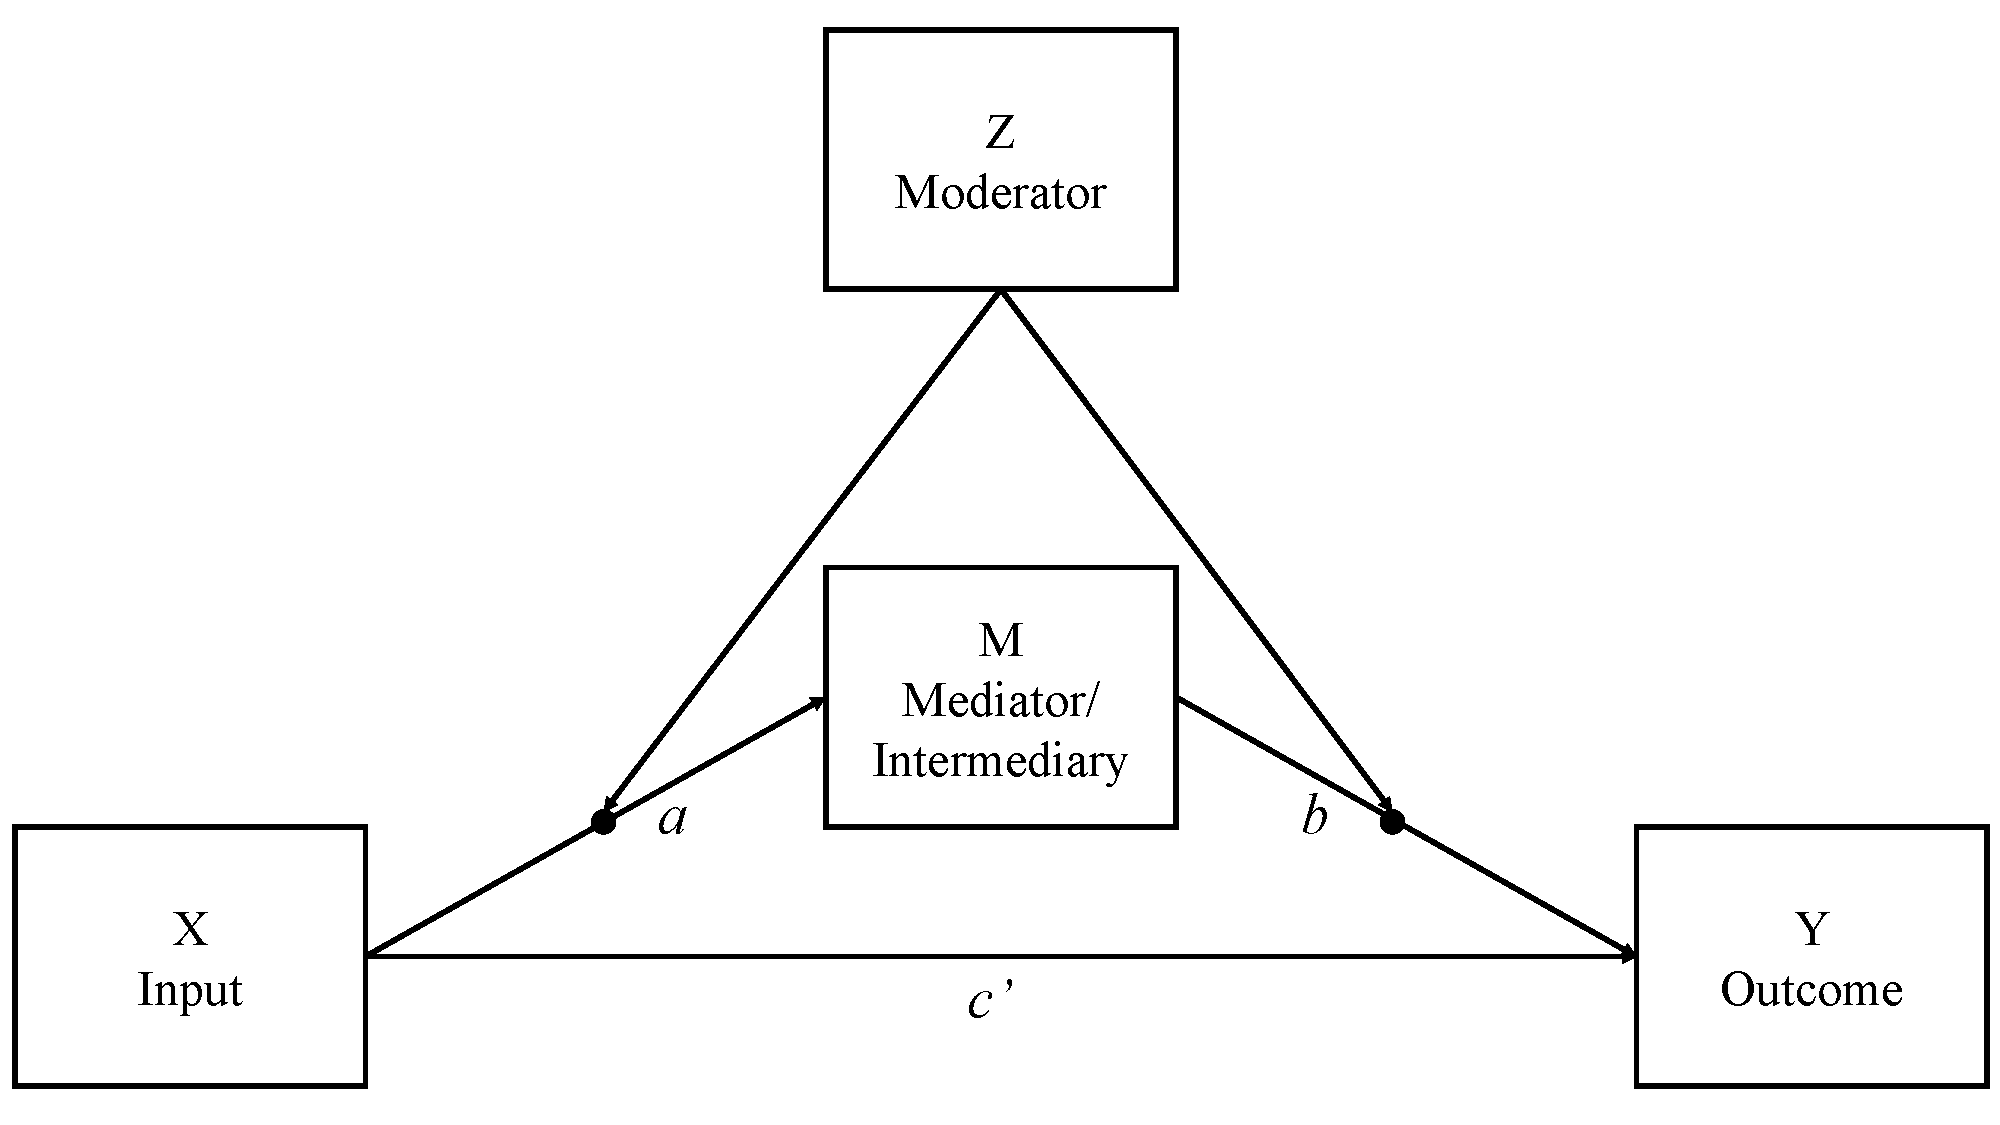
\includegraphics[width=0.95\textwidth]{figures/modABwithZConceptual.pdf}
  \end{figure}
  
\end{frame}



\begin{frame}{Another Example}
  
  The preceding conceptual diagram corresponds to the following
  analytic diagram: 
  \vb
  \begin{figure}
    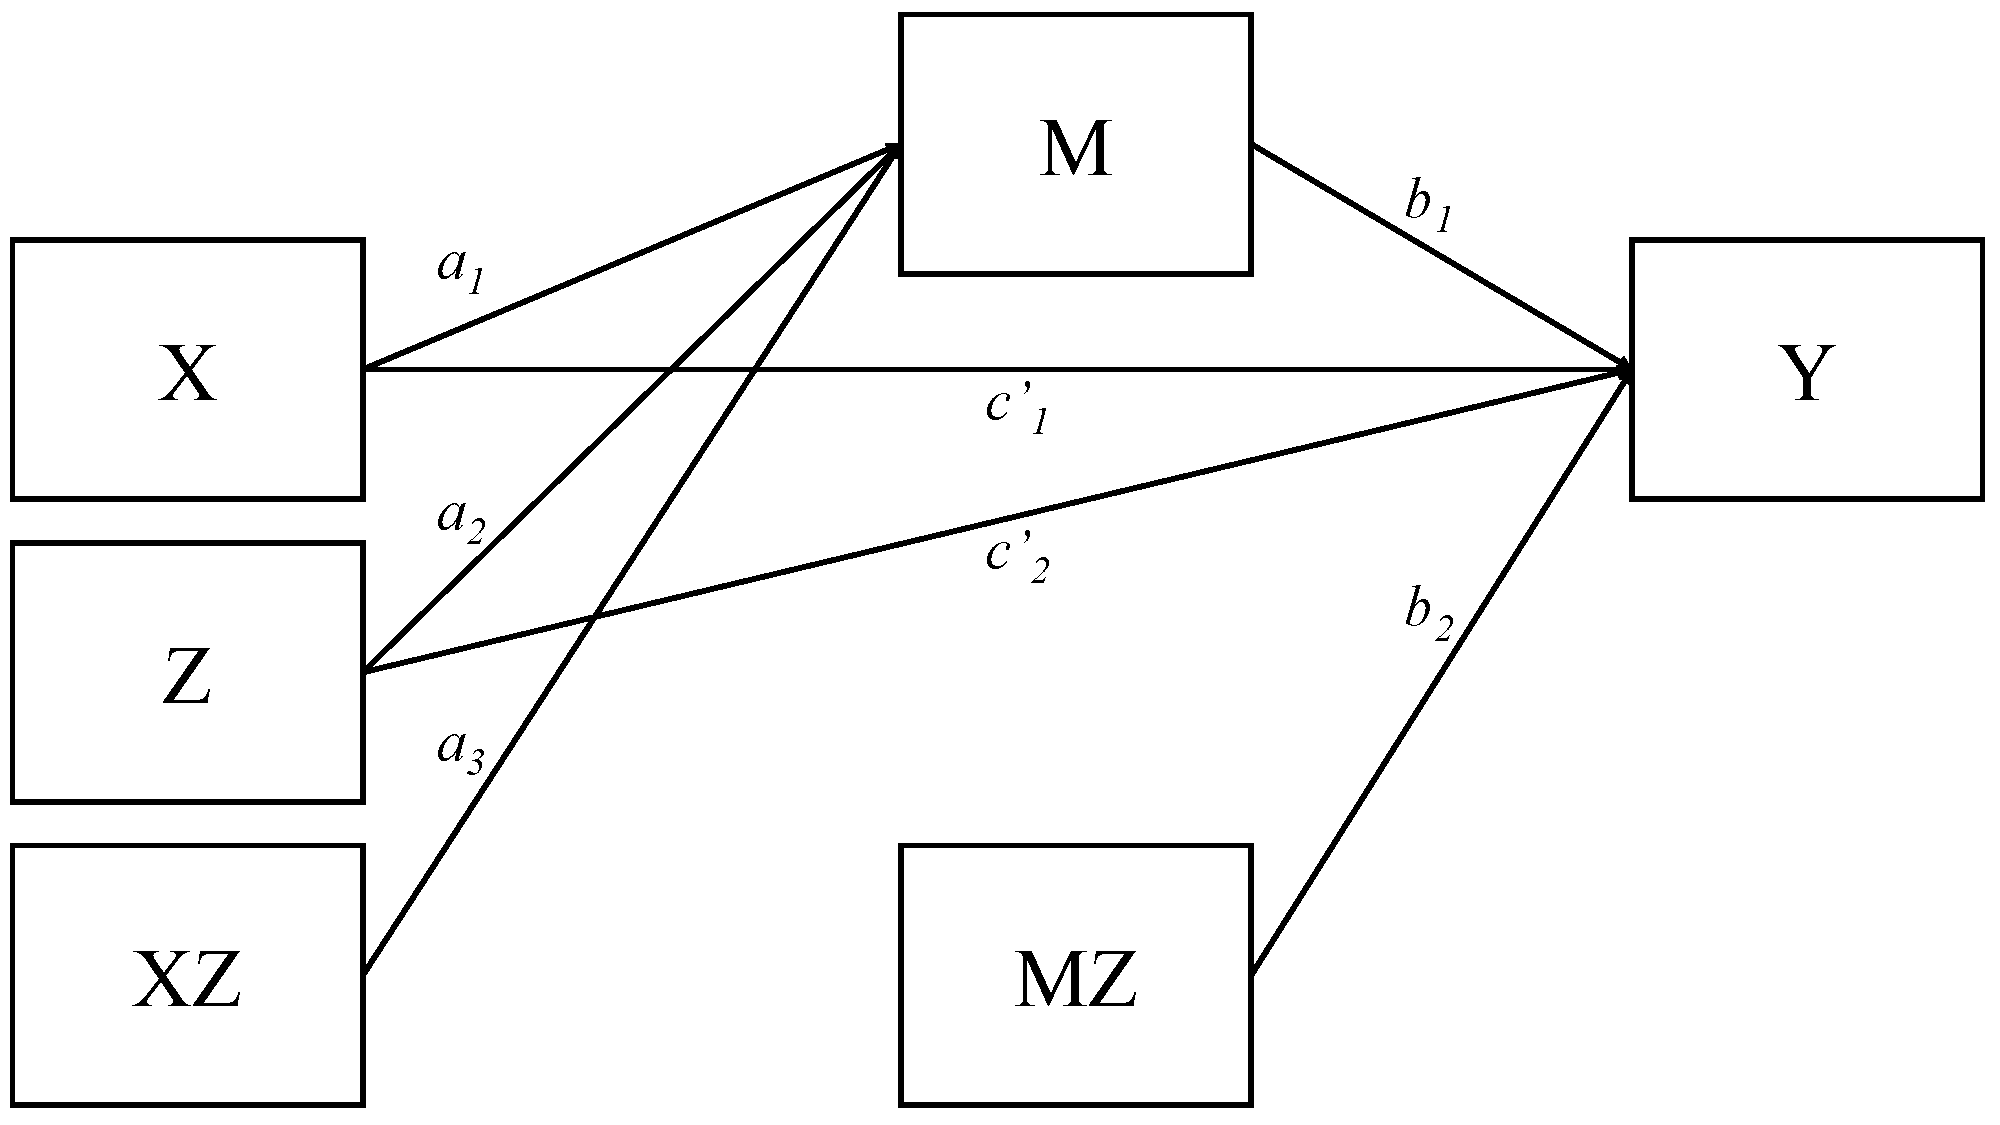
\includegraphics[width=0.95\textwidth]{figures/modABwithZAnalytic.pdf}
  \end{figure}
  
\end{frame}



\begin{frame}{Another Example}
  
  This analytic diagram implies the following equations:
  \begin{align}
    Y &= i_1 + c_1'X + c_2'Z + b_1M + b_2MZ + e_Y \label{eq4}\\
    M &= i_2 + a_1X + a_2Z + a_3XZ + e_M \label{eq5}
  \end{align}
  \pause
  The direct effect is still unconditional:
  \begin{align*}
    DE = c_1'
  \end{align*}
  \pause 
  The indirect effect is conditional on $Z$ due to the
  $a$ and $b$ paths being moderated by $Z$.\\ 
  \va 
  \pause 
  We can rearrange Equations \ref{eq4} and \ref{eq5} to get:
  \begin{align*}
    Y &= i_1 + c_2'Z + \left( b_1 + b_2Z \right)M + e_Y\\
    M &= i_2 + a_2Z + \left( a_1 + a_3Z \right)X + e_M
  \end{align*}
  So, the conditional indirect effect is defined by the following
  product:
  \begin{align*}
    IE = \left(a_1 + a_3Z \right) \left(b_1 + b_2Z \right)
  \end{align*}
  
\end{frame}



\begin{frame}{Another Example}
  
  A conditional indirect effect can arise when the $a$ and $b$ paths
  are moderated by separate variables: 
  \vb
  \begin{figure}
    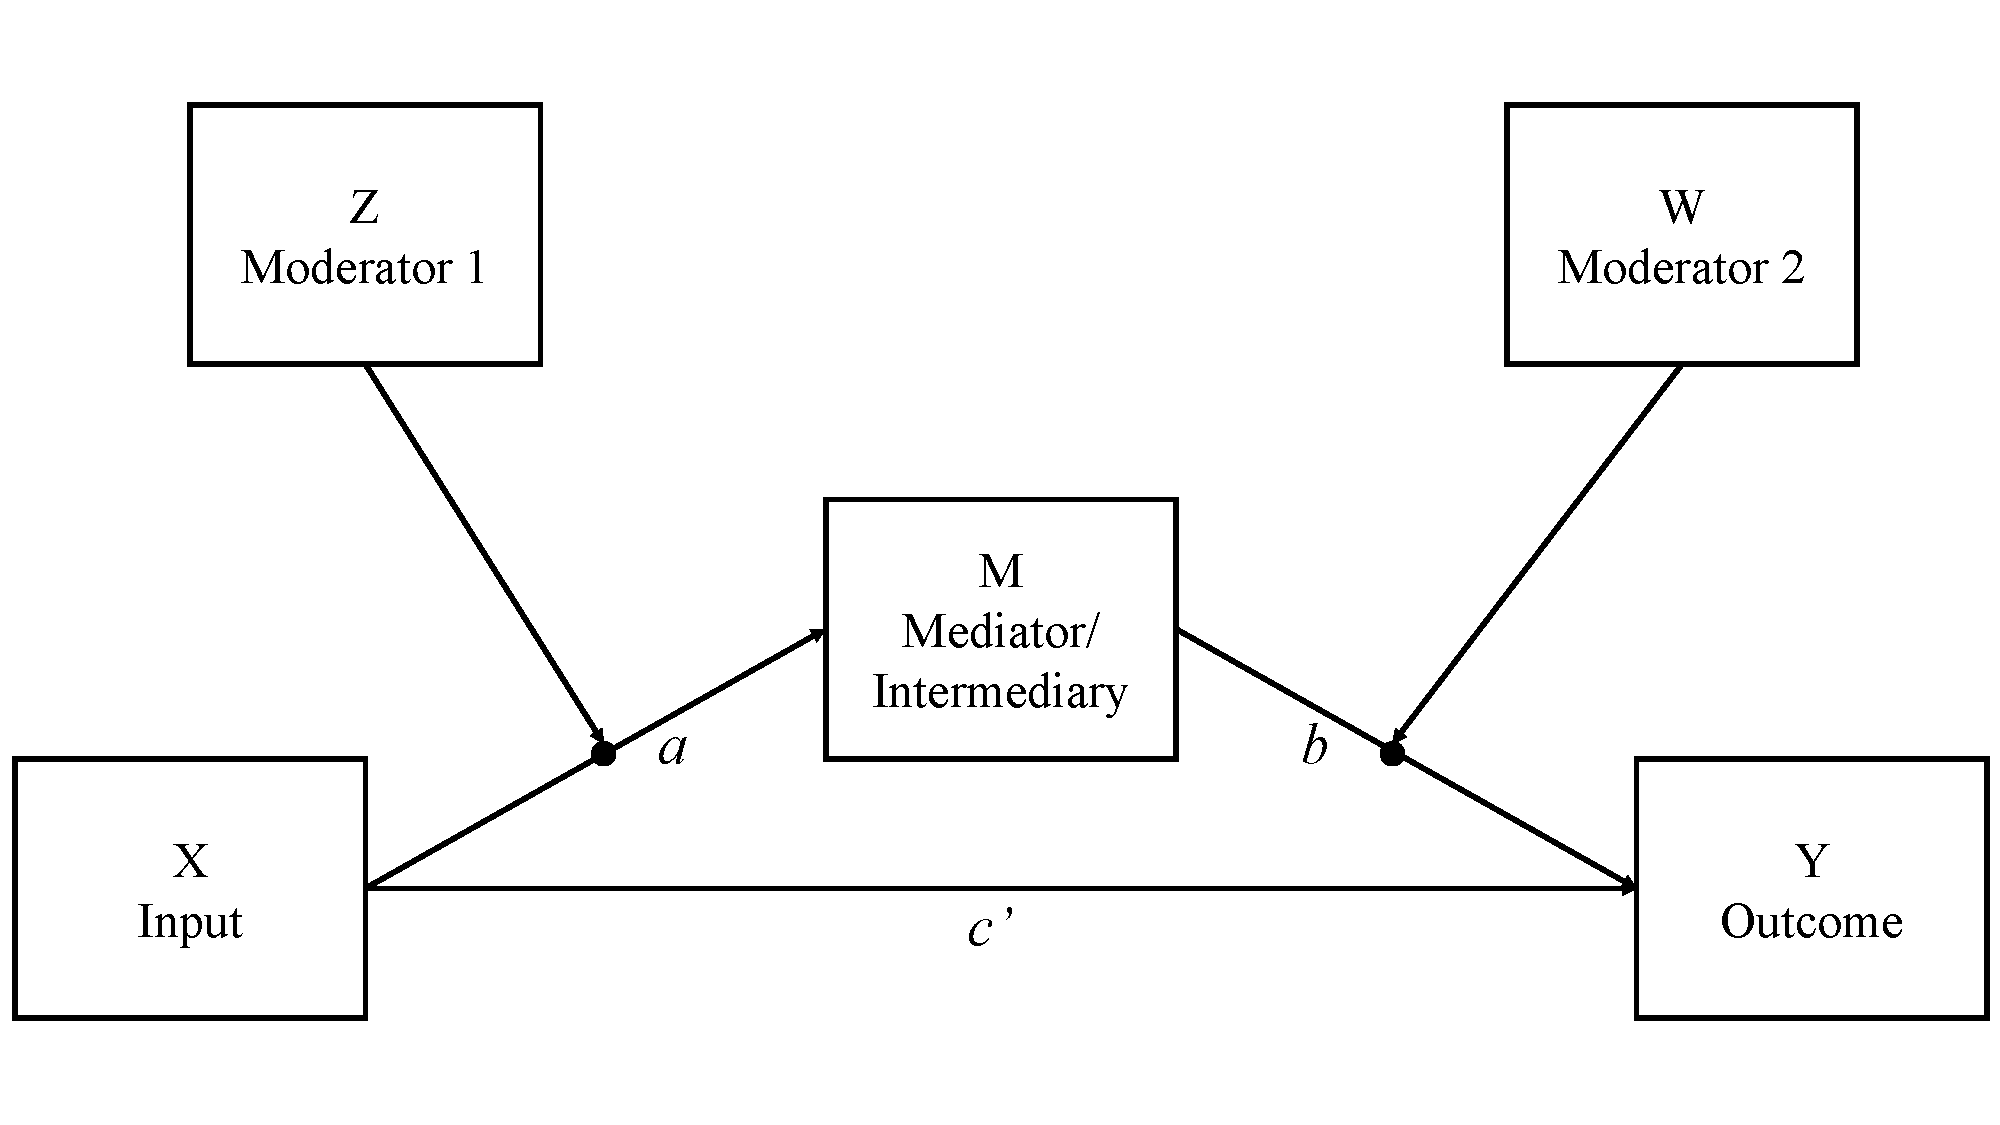
\includegraphics[width=0.95\textwidth]{figures/modAwithZ_BwithWConceptual.pdf}
  \end{figure}
  
\end{frame}



\begin{frame}{Another Example}
  
  The preceding conceptual diagram corresponds to the following
  analytic diagram: 
  \vb
  \begin{figure}
    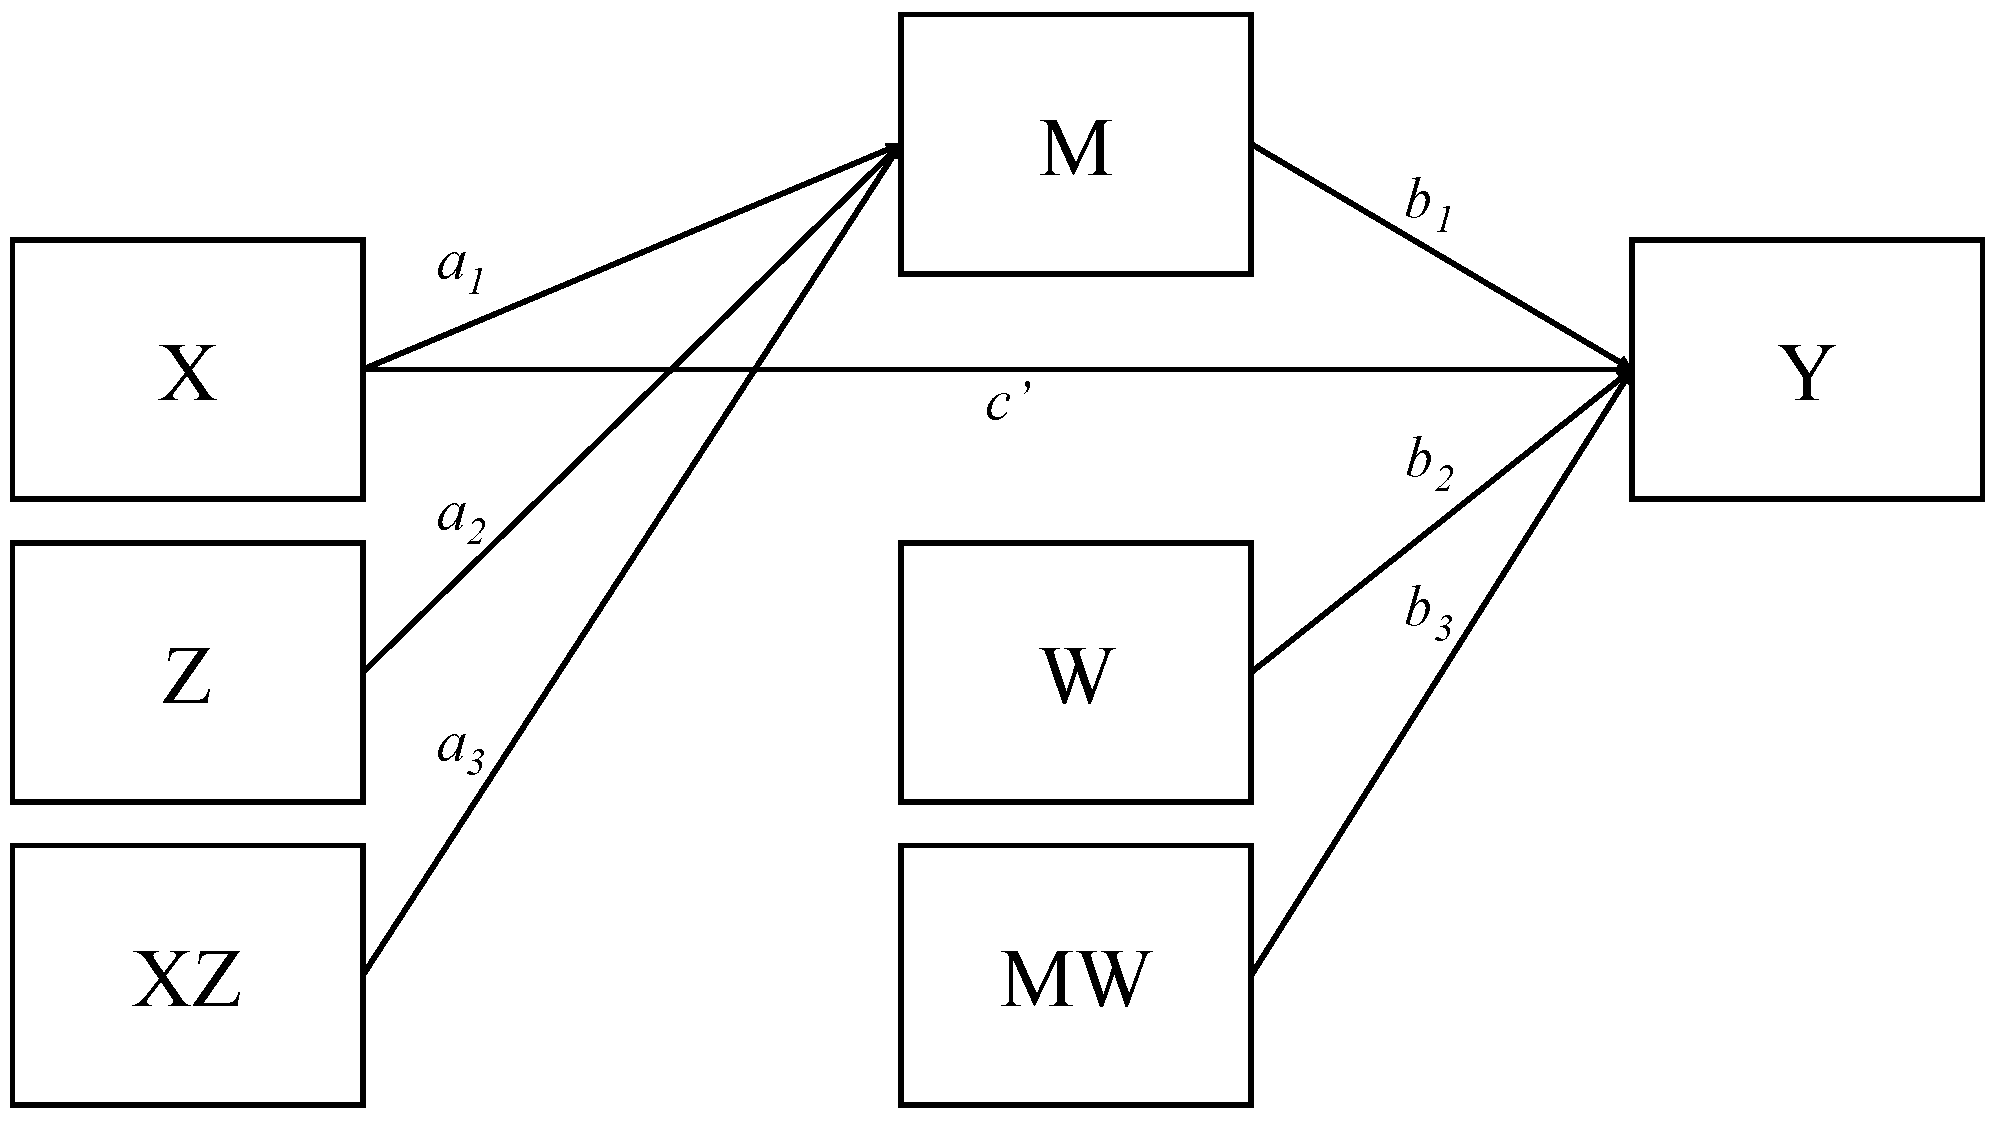
\includegraphics[width=0.95\textwidth]{figures/modAwithZ_BwithWAnalytic.pdf}
  \end{figure}
  
\end{frame}



\begin{frame}{Another Example}
  
  This analytic diagram implies the following equations:
  \begin{align}
    Y &= i_1 + c'X + b_1M + b_2W + b_3MW + e_Y \label{eq6}\\
    M &= i_2 + a_1X + a_2Z + a_3XZ + e_M \label{eq7}
  \end{align}
  \pause
  The direct effect is still unconditional:
  \begin{align*}
    DE = c'
  \end{align*}
  \pause The indirect effect is now conditional on both $Z$ and $W$
  since these variables moderate the $a$ and $b$ paths,
  respectively.\\ 
  \va 
  \pause 
  We can rearrange Equations \ref{eq6} and \ref{eq7} to get:
  \begin{align*}
    Y &= i_1 + b_2W + \left( b_1 + b_3W \right)M + e_Y\\
    M &= i_2 + a_2Z + \left( a_1 + a_3Z \right)X + e_M
  \end{align*}
  So, the conditional indirect effect is defined by the following
  product:
  \begin{align*}
    IE = \left(a_1 + a_3Z \right) \left(b_1 + b_3W \right)
  \end{align*}
  
\end{frame}




\begin{frame}{Another Example}
  
  We could have conditional indirect and direct effects due to
  moderation by a single variable: 
  \vb
  \begin{figure}
    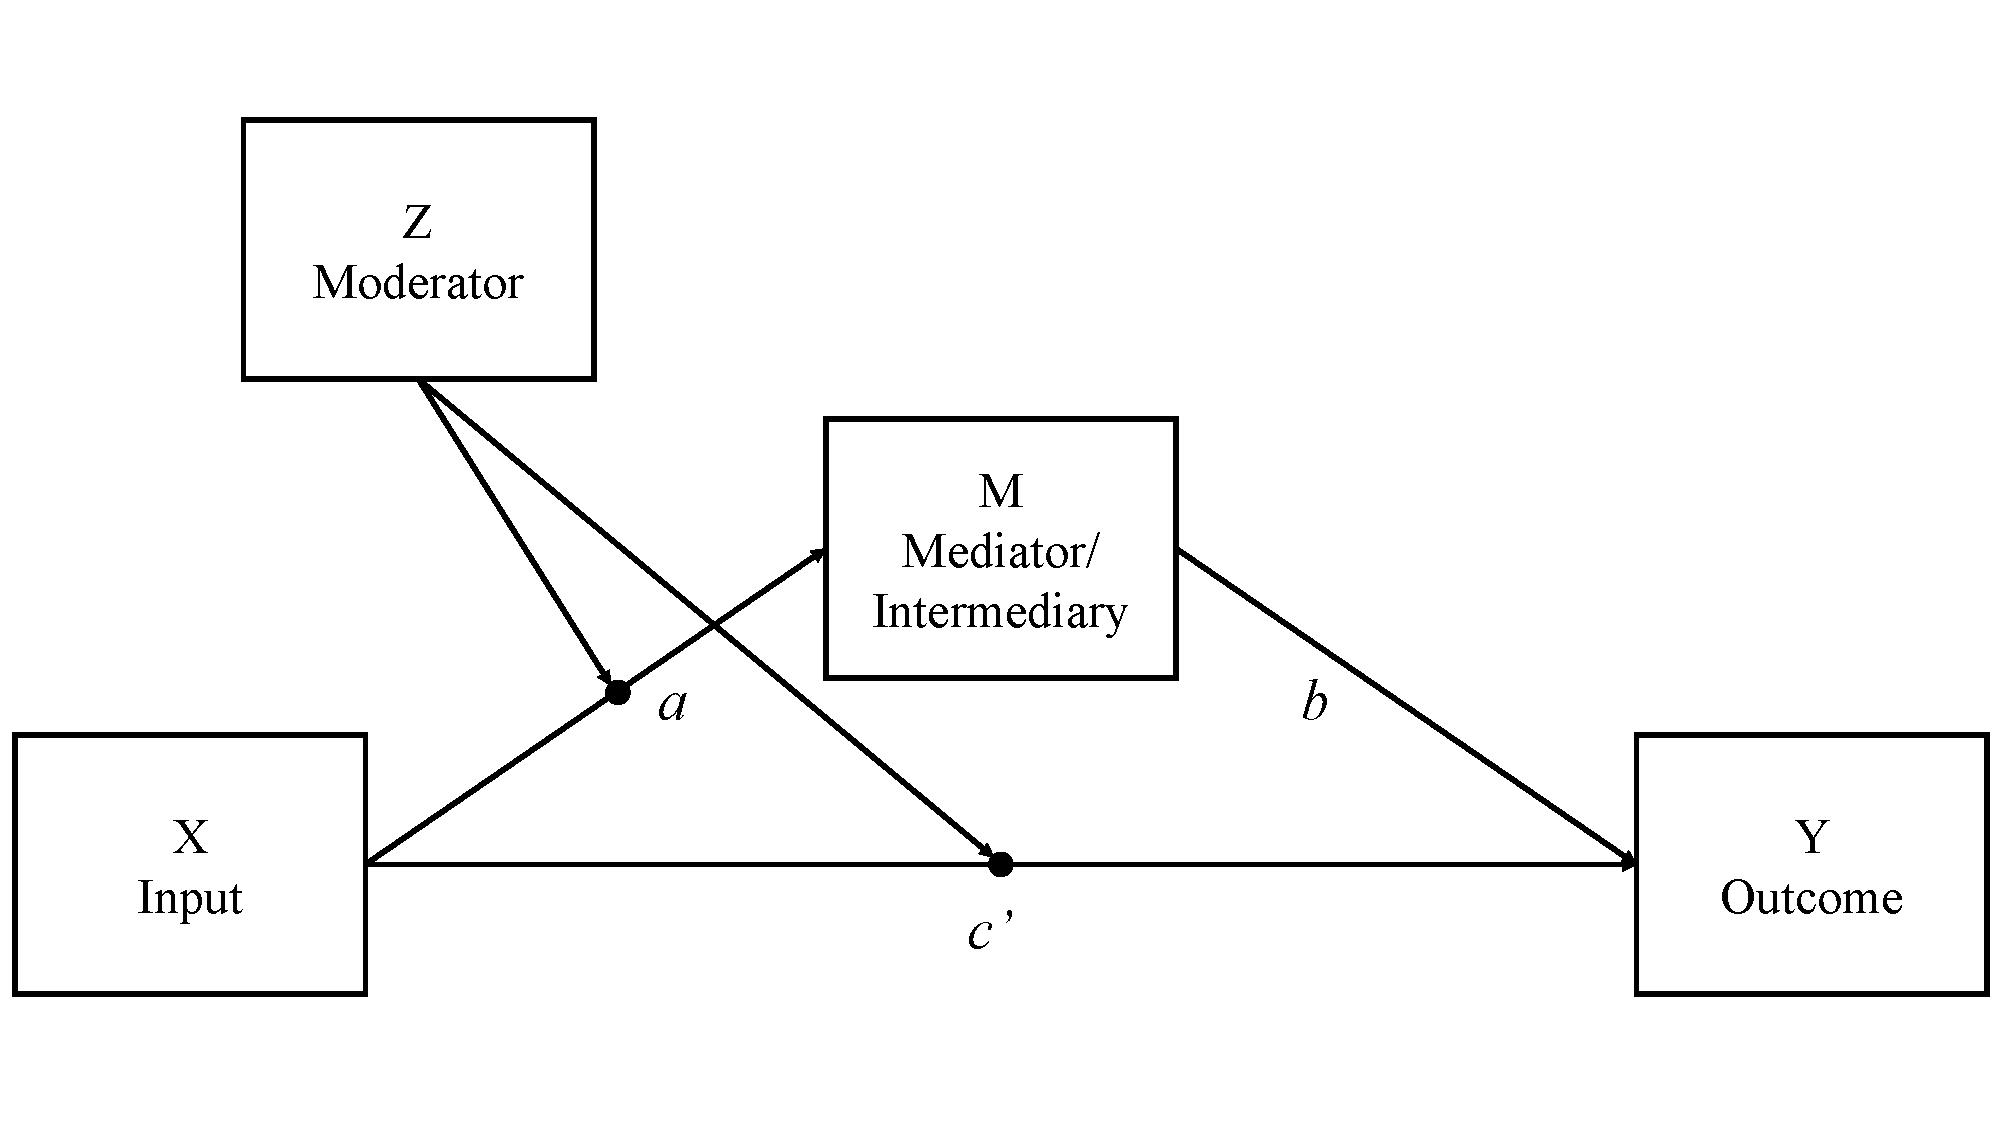
\includegraphics[width=0.95\textwidth]{figures/modACwithZConceptual.pdf}
  \end{figure}
  
\end{frame}



\begin{frame}{Another Example}
  
  The preceding conceptual diagram corresponds to the following
  analytic diagram: 
  \vb
  \begin{figure}
    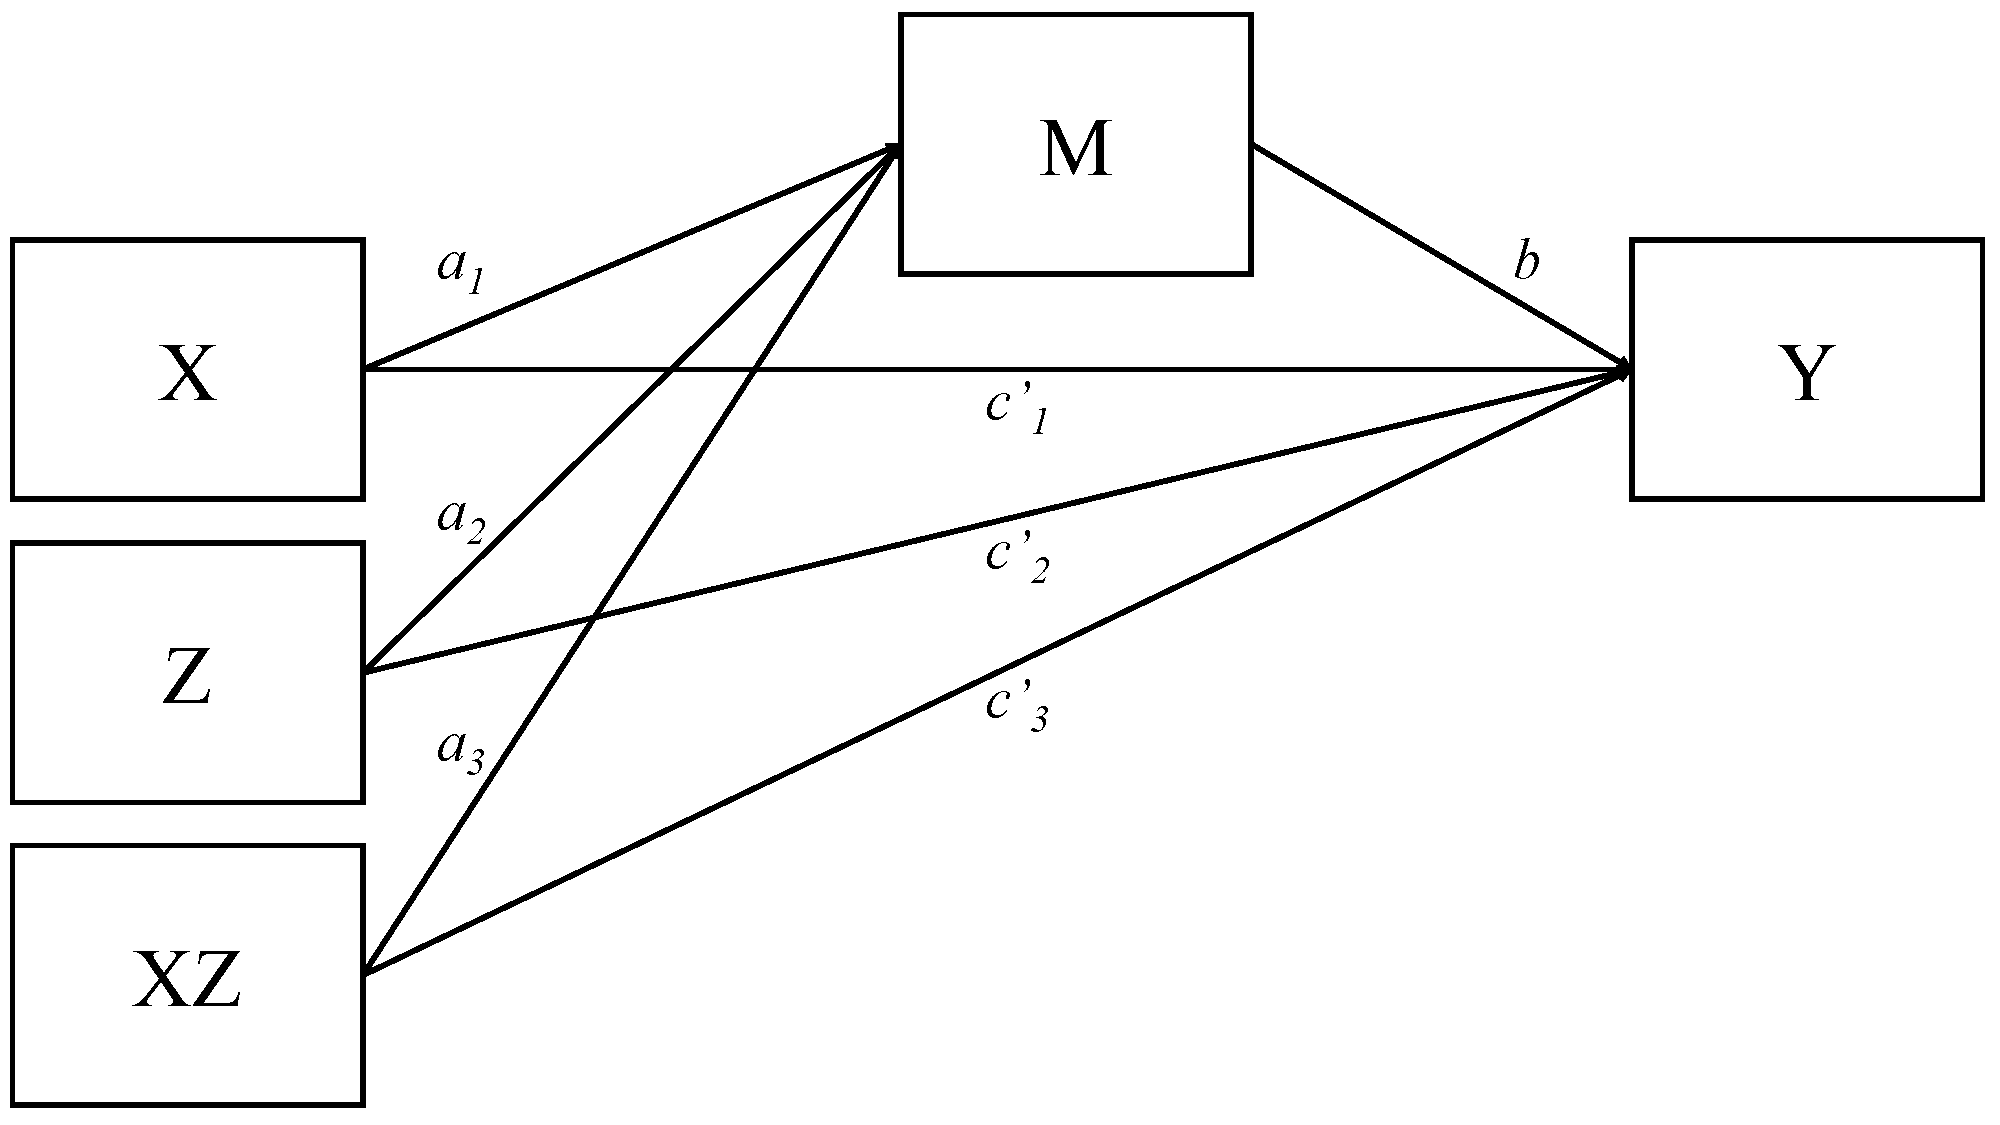
\includegraphics[width=0.95\textwidth]{figures/modACwithZAnalytic.pdf}
  \end{figure}
  
\end{frame}



\begin{frame}{Another Example}
  
  This analytic diagram implies the following equations:
  \begin{align}
    Y &= i_1 + bM + c_1'X + c_2'Z + c_3'XZ + e_Y \label{eq8}\\
    M &= i_2 + a_1X + a_2Z + a_3XZ + e_M \label{eq9}
  \end{align}
  \pause 
  Both the direct and indirect effects are now conditional on
  $Z$ since it moderates the $a$ and $c'$ paths.\\ 
  \va 
  \pause 
  We can rearrange Equations \ref{eq8} and \ref{eq9} to get:
  \begin{align*}
    Y &= i_1 + bM + c_2'Z + \left( c_1' + c_3'Z \right)X + e_Y\\
    M &= i_2 + a_2Z + \left( a_1 + a_3Z \right)X + e_M
  \end{align*}
  So, the conditional direct and indirect effects are defined by the
  following:
  \begin{align*}
    DE &= c_1' + c_3'Z\\
    IE &= \left(a_1 + a_3Z \right) b
  \end{align*}
  
\end{frame}



\begin{frame}{Another Example}
  
  We could have one moderator of the $a$, $b$, and $c'$ paths inducing
  conditional indirect and direct effects: 
  \vb
  \begin{figure}
    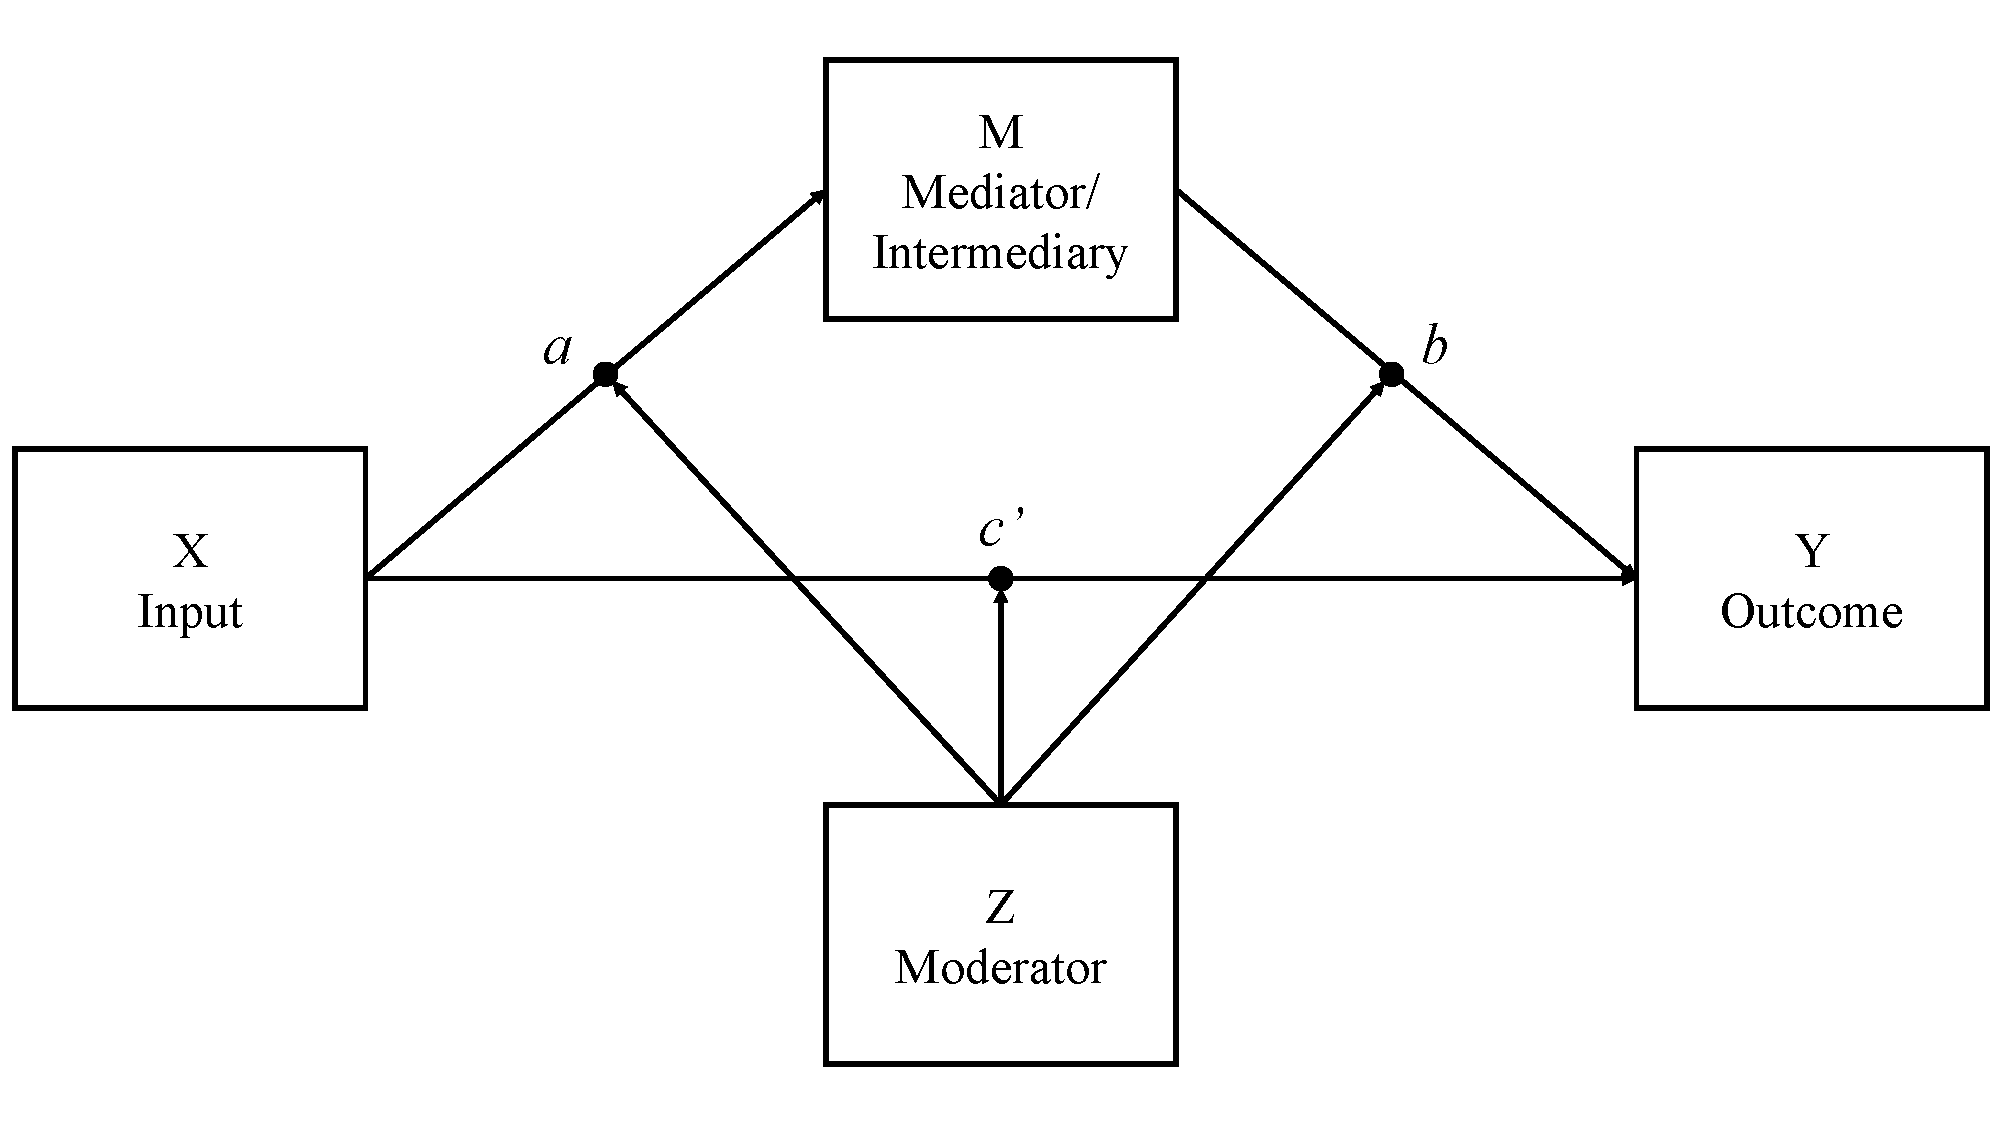
\includegraphics[width=0.95\textwidth]{figures/modABCwithZConceptual.pdf}
  \end{figure}
  
\end{frame}



\begin{frame}{Another Example}
  
  The preceding conceptual diagram corresponds to the following
  analytic diagram: 
  \vb
  \begin{figure}
    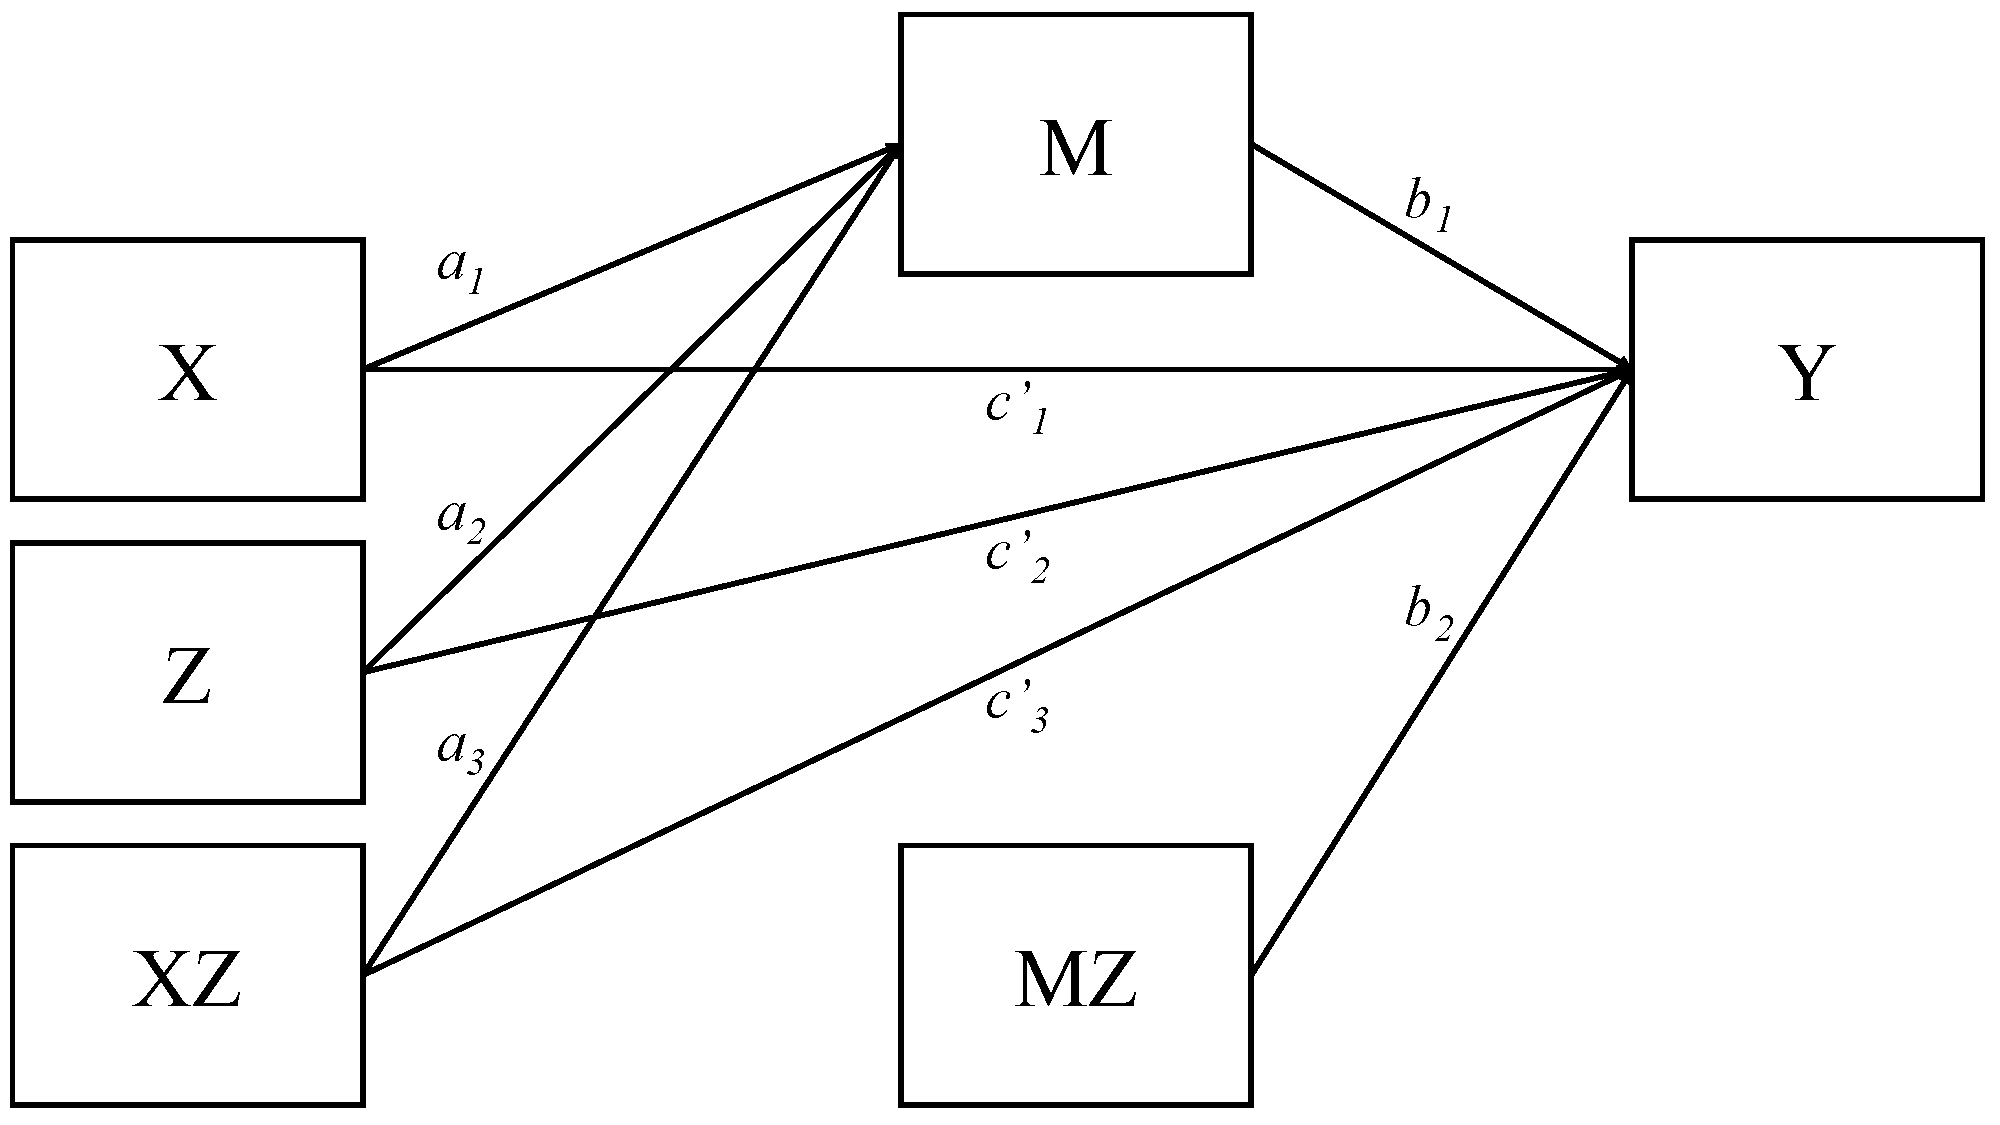
\includegraphics[width=0.95\textwidth]{figures/modABCwithZAnalytic.pdf}
  \end{figure}
  
\end{frame}



\begin{frame}{Another Example}
  
  This analytic diagram implies the following equations:
  \begin{align}
    Y &= i_1 + b_1M + c_1'X + c_2'Z + b_2MZ + c_3'XZ + e_Y \label{eq10}\\
    M &= i_2 + a_1X + a_2Z + a_3XZ + e_M \label{eq11}
  \end{align}
  \pause 
  Both the direct and indirect effects are again conditional on
  $Z$ since it moderates the $a$, $b$, and $c'$ paths.\\ 
  \va 
  \pause 
  We can rearrange Equations \ref{eq10} and \ref{eq11} to get:
  \begin{align*}
    Y &= i_1 + c_2'Z + \left( b_1 + b_2Z \right)M + \left( c_1' + c_3'Z \right)X + e_Y\\
    M &= i_2 + a_2Z + \left( a_1 + a_3Z \right)X + e_M
  \end{align*}
  So, the conditional direct and indirect effects are defined by the
  following:
  \begin{align*}
    DE &= c_1' + c_3'Z\\
    IE &= \left(a_1 + a_3Z \right) \left(b_1 + b_2Z \right)
  \end{align*}
  
\end{frame}



\begin{frame}{Another Example}
  
  Or maybe, the $a$, $b$, and $c'$ paths are each moderated by a
  separate variable to induce the conditional indirect and direct
  effects: 
  \vb
  \begin{figure}
    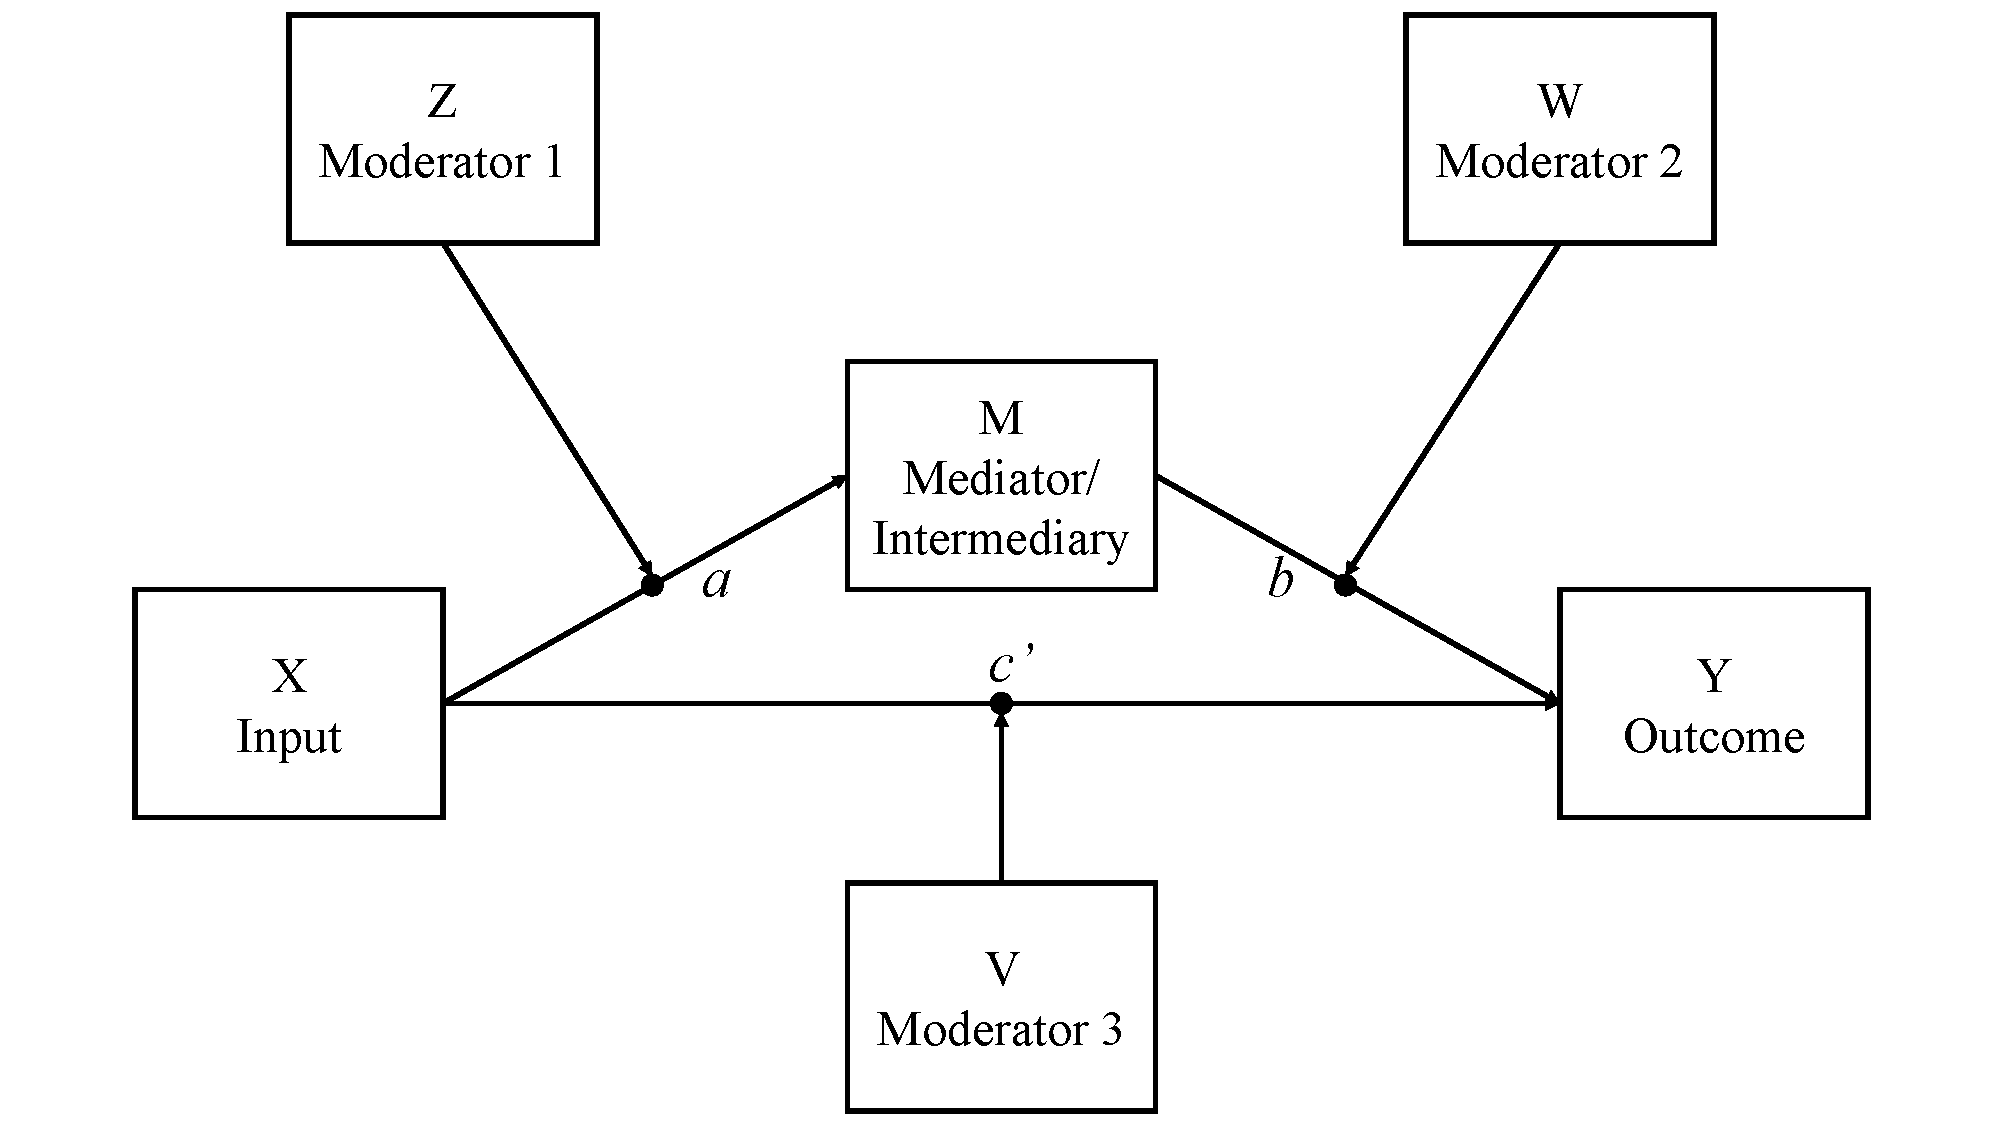
\includegraphics[width=0.95\textwidth]{figures/modAwithZ_BwithW_CwithVConceptual.pdf}
  \end{figure}
  
\end{frame}



\begin{frame}{Another Example}
  
  The preceding conceptual diagram corresponds to the following
  analytic diagram: 
  \vb
  \begin{figure}
    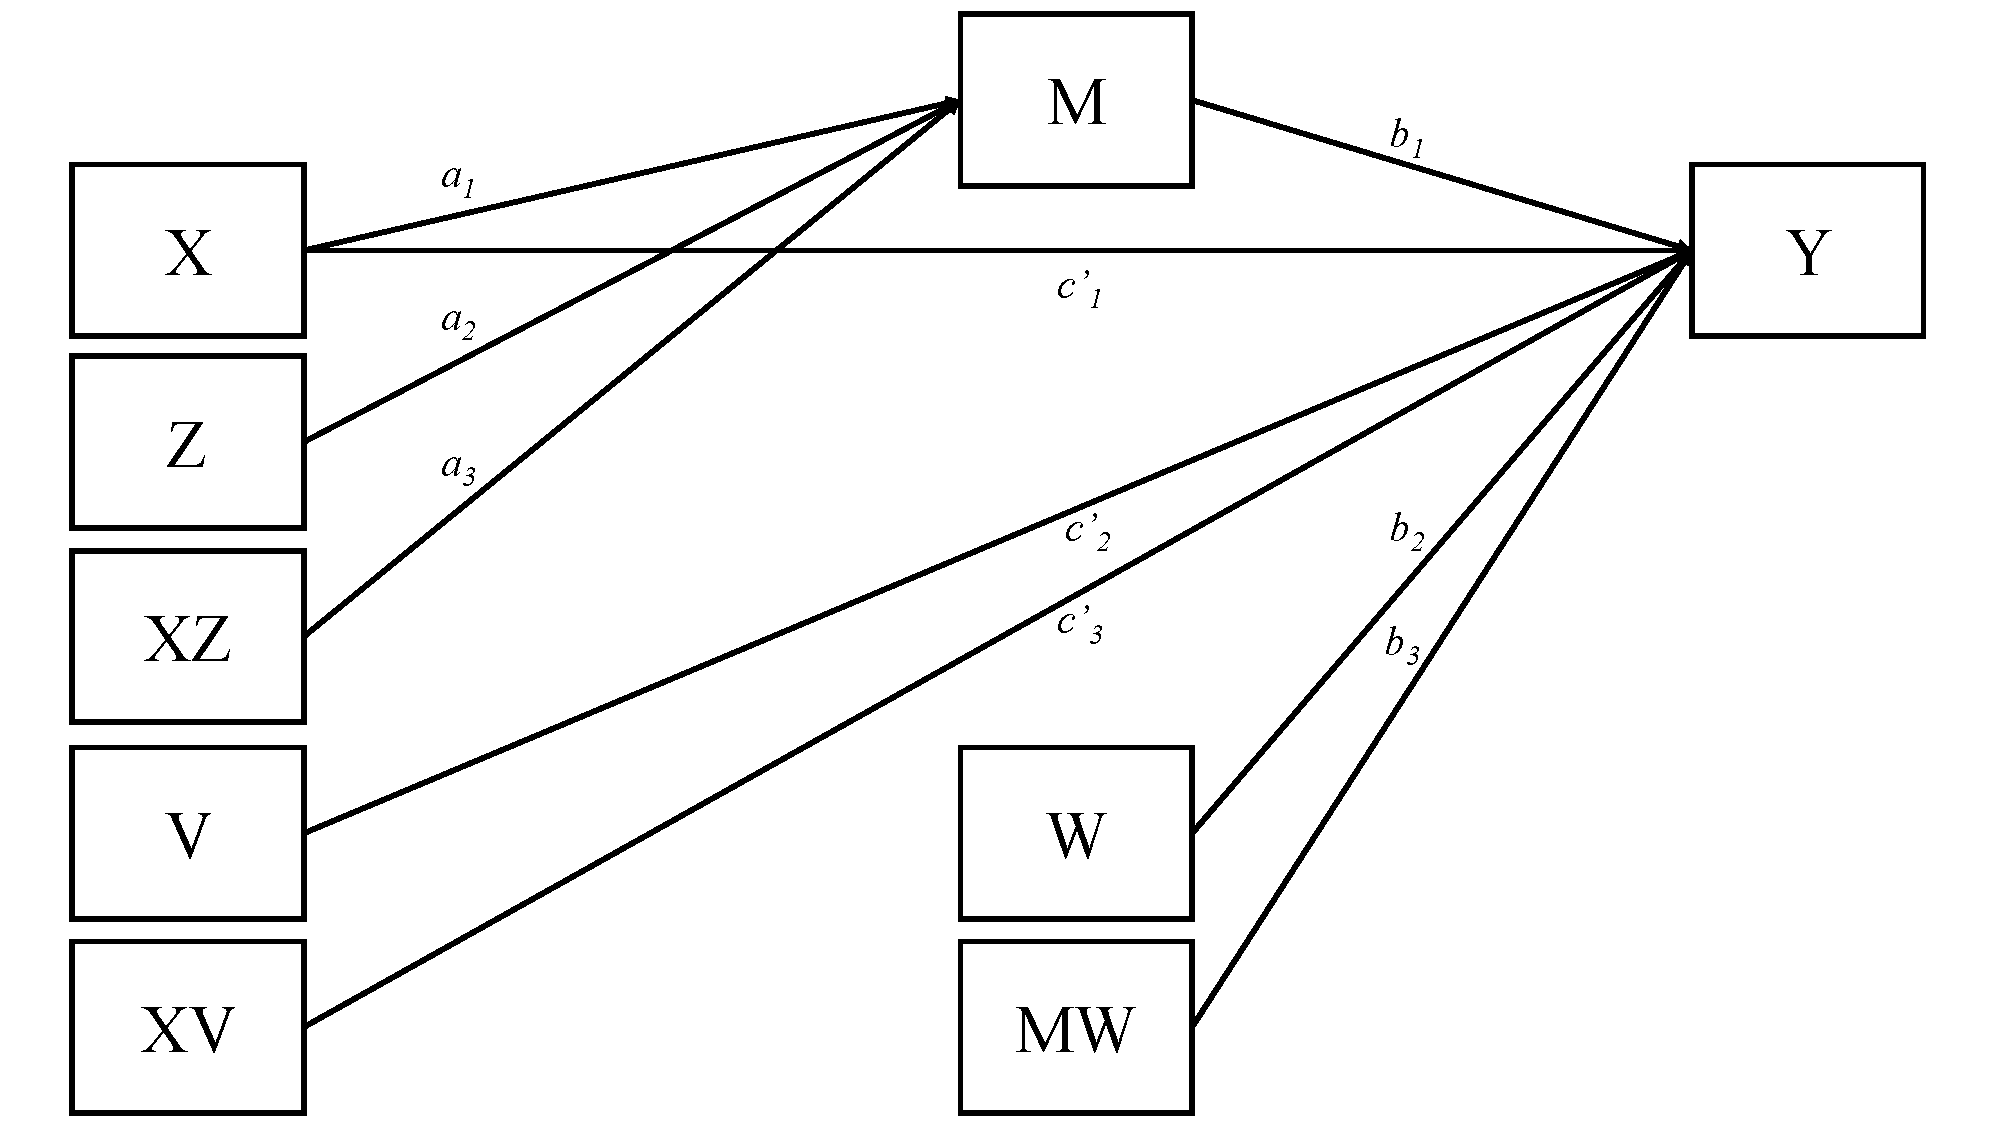
\includegraphics[width=0.95\textwidth]{figures/modAwithZ_BwithW_CwithVAnalytic.pdf}
  \end{figure}
  
\end{frame}



\begin{frame}{Another Example}
  
  This analytic diagram implies the following equations:
  \begin{align*}
    Y &= i_1 + b_1M + b_2W + c_1'X + c_2'V + c_3'XV + b_3MW + e_Y\\
    M &= i_2 + a_1X + a_2Z + a_3XZ + e_M 
  \end{align*}
  \pause 
  The direct effect is now conditional on $V$, while the
  indirect effect is conditional on $Z$ and $W$.\\ 
  \va 
  \pause 
  We can rearrange the preceding equations to get:
  \begin{align*}
    Y &= i_1 + b_2W + c_2'V + \left( b_1 + b_2W \right)M + \left( c_1' + c_3'V \right)X + e_Y\\
    M &= i_2 + a_2Z + \left( a_1 + a_3Z \right)X + e_M
  \end{align*}
  So, the conditional direct and indirect effects are defined by the
  following:
  \begin{align*}
    DE &= c_1' + c_3'V\\
    IE &= \left(a_1 + a_3Z \right) \left(b_1 + b_3W \right)
  \end{align*}
  
\end{frame}



\begin{frame}{Example}
  
  Okay, let's do an example analysis.\\ 
  \va 
  We'll start by fitting the following simple indirect effects 
  model to the \texttt{bfi} data from the \textbf{psych} package: 
  \vb
  \begin{figure}
    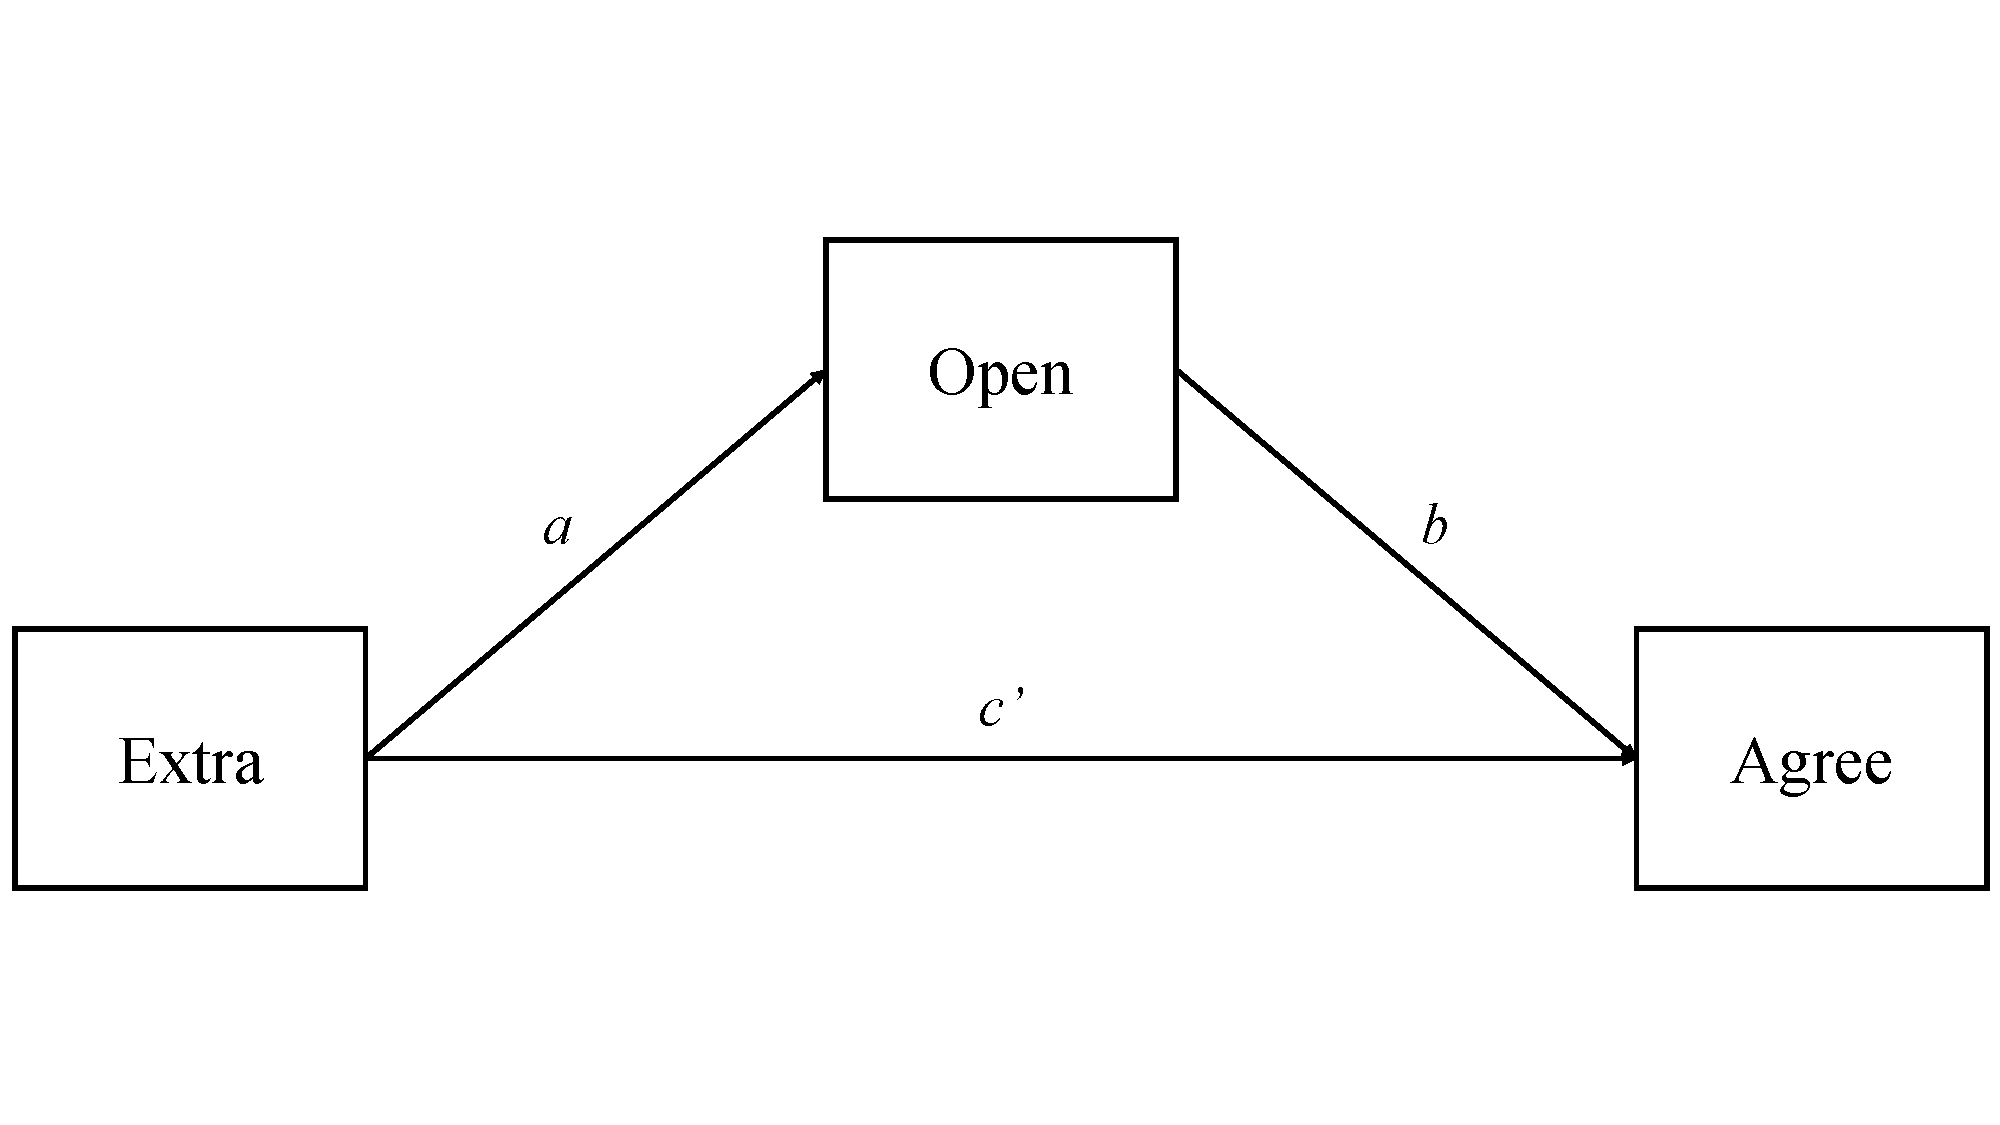
\includegraphics[width=0.95\textwidth]{figures/example1.pdf}
  \end{figure}
  
\end{frame}



\begin{frame}[allowframebreaks]{Example}
  
\begin{Schunk}
\begin{Sinput}
 library(lavaan)
 dataDir <- "../data/"
 dat1 <- readRDS(paste0(dataDir, "adamsKlpsData.rds"))
 ## Specify the CFA model:
 mod1.1 <- "
 merit =~ meritP1 + meritP2 + meritP3
 policy =~ policyP1 + policyP2 + policyP3
 "
 ## Fit the CFA and check model:
 out1.1 <- cfa(mod1.1, data = dat1, std.lv = TRUE)
 ## Check model fit:
 round(fitMeasures(out1.1)[c("chisq", "df", "pvalue", "cfi", 
                             "tli", "rmsea", "srmr")], 4)
\end{Sinput}
\begin{Soutput}
  chisq      df  pvalue     cfi     tli   rmsea    srmr 
16.8695  8.0000  0.0315  0.9215  0.8529  0.1129  0.0653 
\end{Soutput}
\begin{Sinput}
 summary(out1.1)
\end{Sinput}
\begin{Soutput}
lavaan (0.5-20) converged normally after  22 iterations

  Number of observations                            87

  Estimator                                         ML
  Minimum Function Test Statistic               16.869
  Degrees of freedom                                 8
  P-value (Chi-square)                           0.031

Parameter Estimates:

  Information                                 Expected
  Standard Errors                             Standard

Latent Variables:
                   Estimate  Std.Err  Z-value  P(>|z|)
  merit =~                                            
    meritP1           0.690    0.134    5.155    0.000
    meritP2           0.968    0.142    6.830    0.000
    meritP3           0.748    0.137    5.458    0.000
  policy =~                                           
    policyP1          0.851    0.186    4.570    0.000
    policyP2          0.996    0.167    5.967    0.000
    policyP3          1.121    0.177    6.339    0.000

Covariances:
                   Estimate  Std.Err  Z-value  P(>|z|)
  merit ~~                                            
    policy           -0.336    0.131   -2.563    0.010

Variances:
                   Estimate  Std.Err  Z-value  P(>|z|)
    meritP1           0.865    0.165    5.248    0.000
    meritP2           0.445    0.201    2.211    0.027
    meritP3           0.833    0.172    4.857    0.000
    policyP1          1.836    0.324    5.671    0.000
    policyP2          0.942    0.256    3.683    0.000
    policyP3          0.857    0.297    2.882    0.004
    merit             1.000                           
    policy            1.000                           
\end{Soutput}
\end{Schunk}


\end{frame}


\begin{frame}{Example}
  
  Maybe we suspect that \emph{conscientiousness} moderates the effect of
  \emph{openness} on \emph{agreeableness} (i.e., the $b$ path).\\
  \va
  We can assess this conditional process via the following model:\\ 
  \vb
  \begin{figure}
    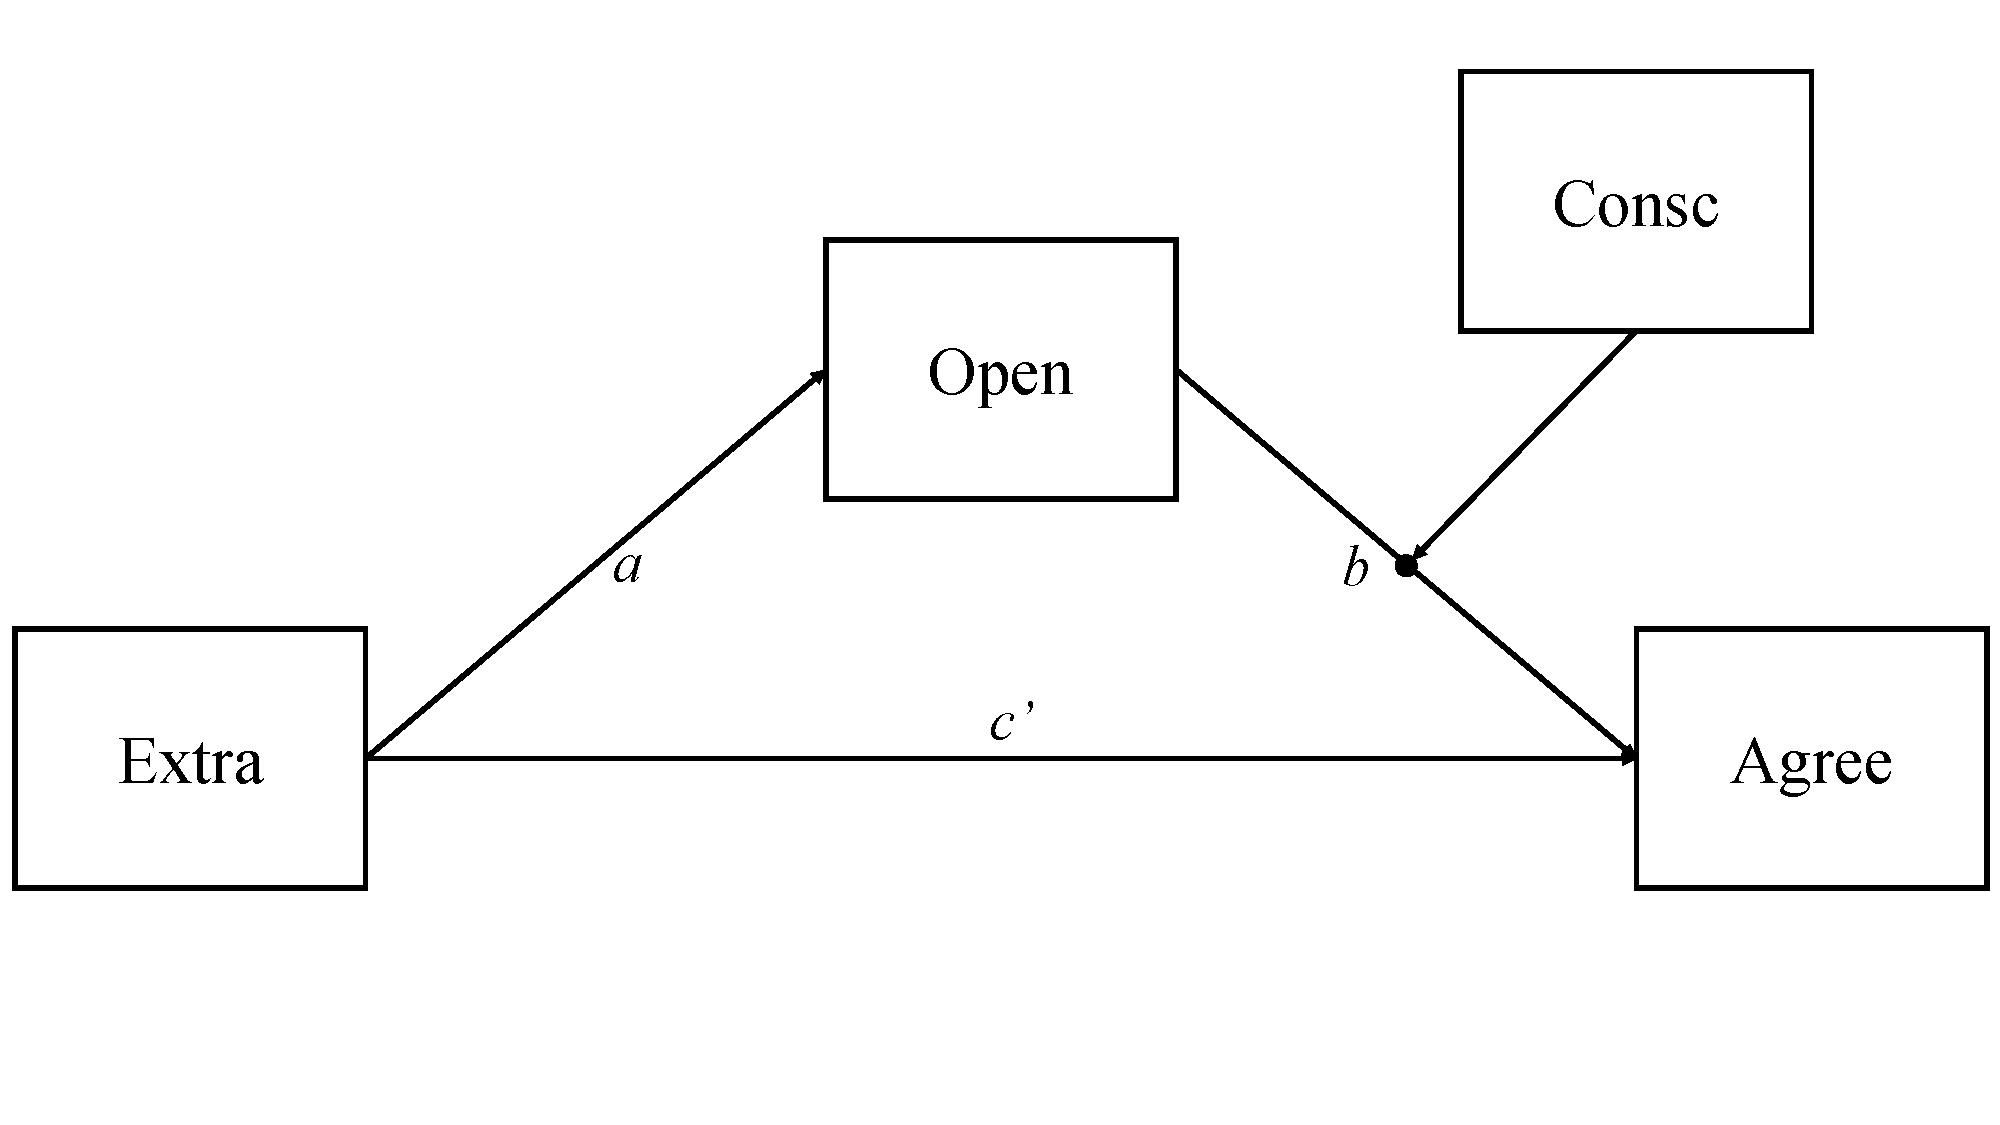
\includegraphics[width=0.95\textwidth]{figures/example2Conceptual.pdf}
  \end{figure}
  
\end{frame}




\begin{frame}{Example}
  
  The preceding conceptual model translates into the following
  analytic model: 
  \vb
  \begin{figure}
    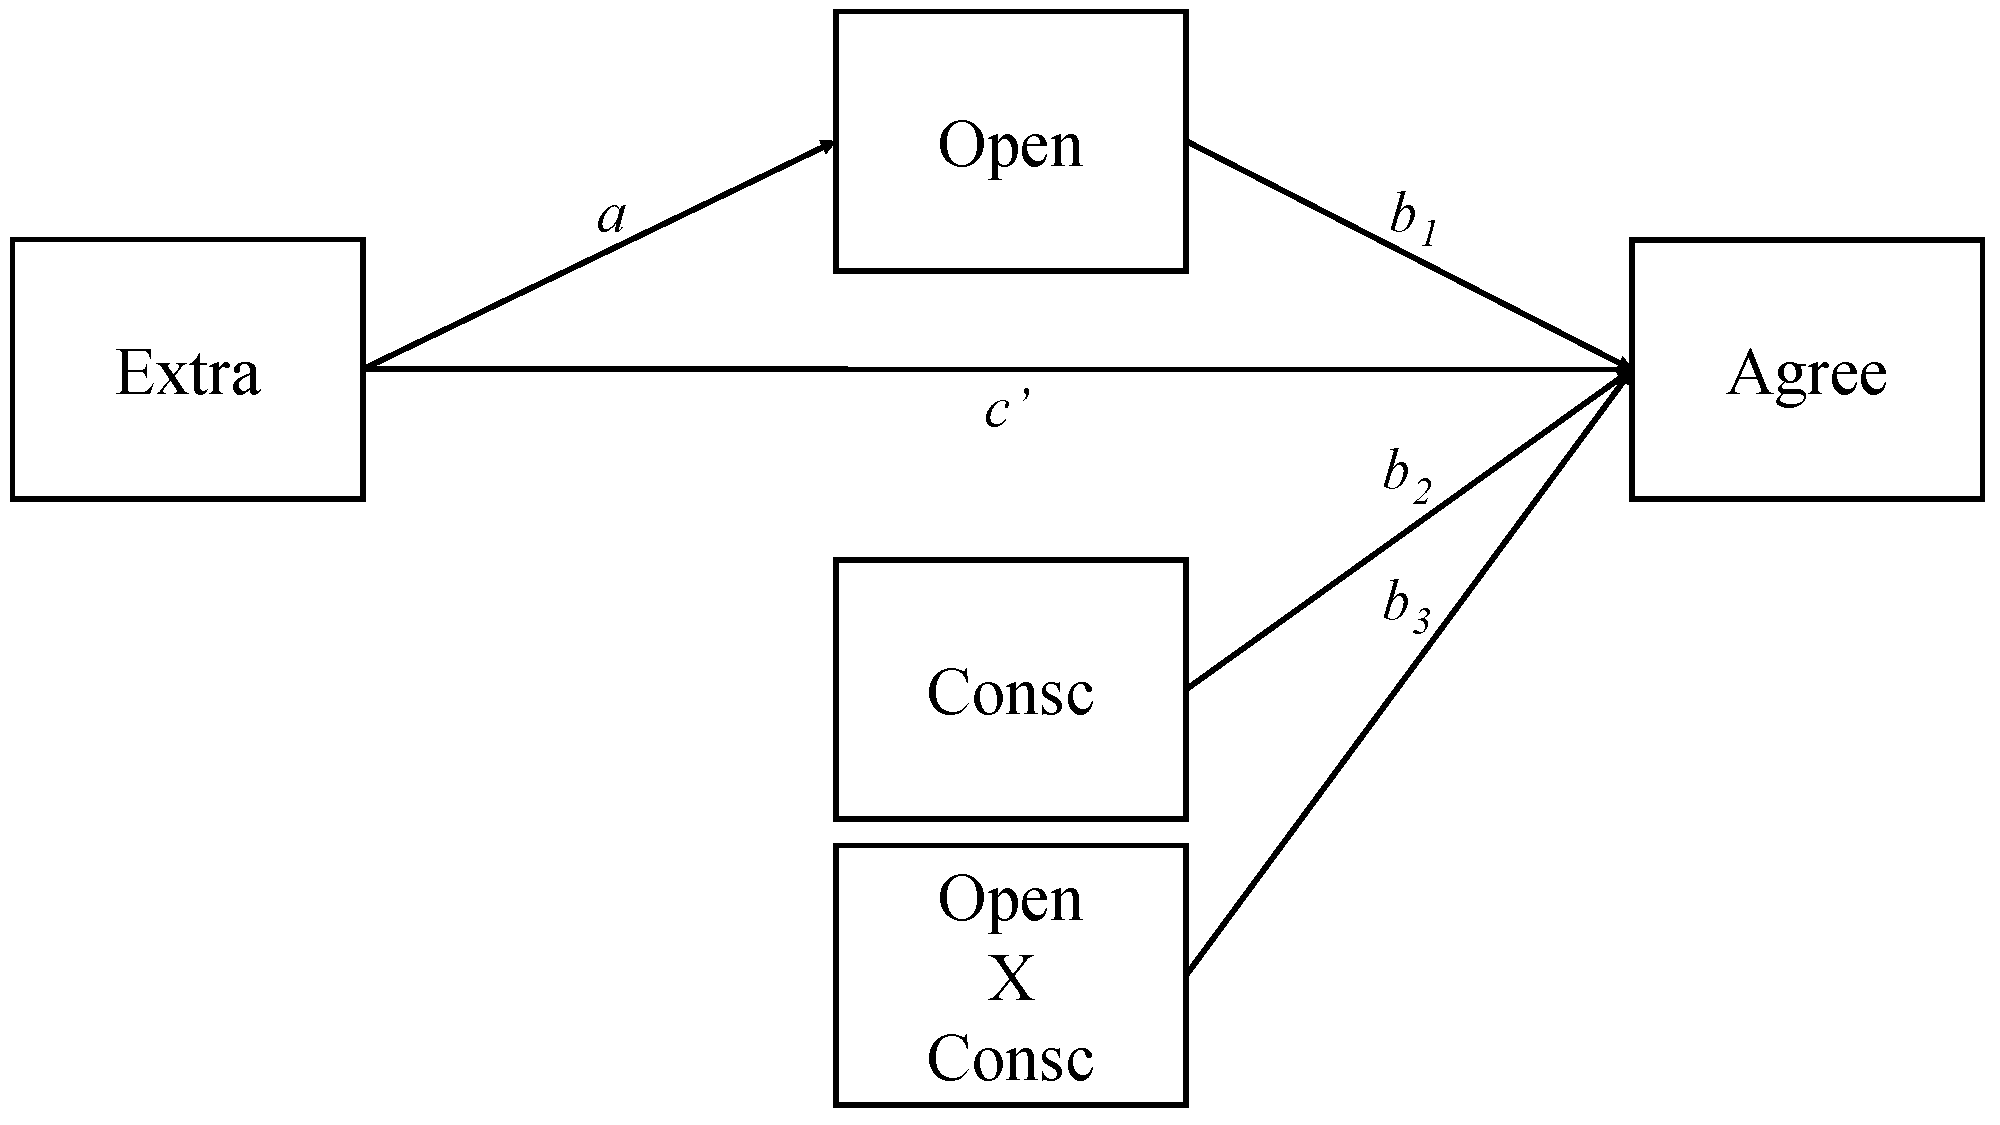
\includegraphics[width=0.95\textwidth]{figures/example2Analytic.pdf}
  \end{figure}
  
\end{frame}



\begin{frame}[allowframebreaks]{Example}
  
\begin{Schunk}
\begin{Sinput}
 round(fitMeasures(out1)[c("chisq", "df", "pvalue", "cfi", 
                           "tli", "rmsea", "srmr")], 3)
\end{Sinput}
\begin{Soutput}
 chisq     df pvalue    cfi    tli  rmsea   srmr 
41.021 24.000  0.017  0.987  0.981  0.038  0.026 
\end{Soutput}
\end{Schunk}


\pagebreak

\begin{Schunk}
\begin{Sinput}
 mod3 <- "
 att3 ~ att2 + b2*conf2 + cp2*horn2
 att2 ~ att1 + b1*conf1 + cp1*horn1
 
 conf3 ~ conf2 + a2*horn2
 conf2 ~ conf1 + a1*horn1
 
 horn3 ~ horn2
 horn2 ~ horn1
 
 horn3 ~~ conf3 + att3
 conf3 ~~ att3
 
 horn2 ~~ conf2 + att2
 conf2 ~~ att2
 
 a1 == a2
 b1 == b2
 cp1 == cp2
 "
 out3 <- sem(mod3, data = dat1)
 summary(out3)
\end{Sinput}
\begin{Soutput}
lavaan (0.5-20) converged normally after  46 iterations

  Number of observations                           500

  Estimator                                         ML
  Minimum Function Test Statistic              294.220
  Degrees of freedom                                18
  P-value (Chi-square)                           0.000

Parameter Estimates:

  Information                                 Expected
  Standard Errors                             Standard

Regressions:
                   Estimate  Std.Err  Z-value  P(>|z|)
  att3 ~                                              
    att2              0.497    0.035   14.234    0.000
    conf2     (b2)    0.098    0.019    5.200    0.000
    horn2    (cp2)    0.083    0.072    1.157    0.247
  att2 ~                                              
    att1              0.530    0.040   13.345    0.000
    conf1     (b1)    0.098    0.019    5.200    0.000
    horn1    (cp1)    0.083    0.072    1.157    0.247
  conf3 ~                                             
    conf2             0.684    0.035   19.602    0.000
    horn2     (a2)    0.493    0.107    4.596    0.000
  conf2 ~                                             
    conf1             0.623    0.032   19.546    0.000
    horn1     (a1)    0.493    0.107    4.596    0.000
  horn3 ~                                             
    horn2             0.826    0.030   27.609    0.000
  horn2 ~                                             
    horn1             0.714    0.024   29.181    0.000

Covariances:
                   Estimate  Std.Err  Z-value  P(>|z|)
  conf3 ~~                                            
    horn3             1.016    0.155    6.556    0.000
  att3 ~~                                             
    horn3             0.322    0.093    3.483    0.000
    conf3             3.574    0.465    7.691    0.000
  conf2 ~~                                            
    horn2             0.836    0.124    6.721    0.000
  att2 ~~                                             
    horn2             0.273    0.083    3.289    0.001
    conf2             2.027    0.400    5.067    0.000

Variances:
                   Estimate  Std.Err  Z-value  P(>|z|)
    att3              6.019    0.381   15.811    0.000
    att2              6.041    0.382   15.811    0.000
    conf3            15.814    1.000   15.811    0.000
    conf2            12.570    0.795   15.811    0.000
    horn3             0.695    0.044   15.811    0.000
    horn2             0.560    0.035   15.811    0.000

Constraints:
                                               |Slack|
    a1 - (a2)                                    0.000
    b1 - (b2)                                    0.000
    cp1 - (cp2)                                  0.000
\end{Soutput}
\begin{Sinput}
 chiDiff <- fitMeasures(out3)["chisq"] -
     fitMeasures(out1)["chisq"]
 dfDiff <- fitMeasures(out3)["df"] -
     fitMeasures(out1)["df"]
 pchisq(chiDiff, dfDiff, lower = FALSE)
\end{Sinput}
\begin{Soutput}
     chisq 
0.02684148 
\end{Soutput}
\end{Schunk}


\pagebreak

\begin{Schunk}
\begin{Sinput}
 mod4 <- "
 att3 ~ att2 + b2*conf2 + cp*horn1
 att2 ~ att1 + b1*conf1
 
 conf3 ~ conf2 + a2*horn2
 conf2 ~ conf1 + a1*horn1
 
 att2 + att3 ~ income
 conf2 + conf3 ~ income 
 horn2 + horn3 ~ income
 
 horn3 ~ horn2
 horn2 ~ horn1
 
 horn3 ~~ conf3 + att3
 conf3 ~~ att3
 
 horn2 ~~ conf2 + att2
 conf2 ~~ att2
 
 ab := a1*b2
 "
 out4 <- sem(mod4, data = dat1, se = "boot", boot = nBoot)
 summary(out4)
\end{Sinput}
\begin{Soutput}
lavaan (0.5-20) converged normally after  63 iterations

  Number of observations                           500

  Estimator                                         ML
  Minimum Function Test Statistic              219.789
  Degrees of freedom                                16
  P-value (Chi-square)                           0.000

Parameter Estimates:

  Information                                 Observed
  Standard Errors                            Bootstrap
  Number of requested bootstrap draws             2000
  Number of successful bootstrap draws            2000

Regressions:
                   Estimate  Std.Err  Z-value  P(>|z|)
  att3 ~                                              
    att2              0.513    0.039   13.099    0.000
    conf2     (b2)    0.022    0.027    0.826    0.409
    horn1     (cp)   -0.119    0.084   -1.418    0.156
  att2 ~                                              
    att1              0.477    0.043   10.980    0.000
    conf1     (b1)    0.084    0.028    3.048    0.002
  conf3 ~                                             
    conf2             0.488    0.041   11.803    0.000
    horn2     (a2)    0.492    0.160    3.076    0.002
  conf2 ~                                             
    conf1             0.543    0.037   14.594    0.000
    horn1     (a1)    0.175    0.146    1.204    0.228
  att2 ~                                              
    income            0.052    0.013    4.108    0.000
  att3 ~                                              
    income            0.057    0.012    4.853    0.000
  conf2 ~                                             
    income            0.110    0.016    6.871    0.000
  conf3 ~                                             
    income            0.148    0.018    8.206    0.000
  horn2 ~                                             
    income            0.016    0.003    5.698    0.000
  horn3 ~                                             
    income            0.013    0.004    3.555    0.000
    horn2             0.780    0.033   23.921    0.000
  horn2 ~                                             
    horn1             0.654    0.026   25.525    0.000

Covariances:
                   Estimate  Std.Err  Z-value  P(>|z|)
  conf3 ~~                                            
    horn3             0.915    0.152    6.020    0.000
  att3 ~~                                             
    horn3             0.322    0.092    3.489    0.000
    conf3             2.971    0.412    7.215    0.000
  conf2 ~~                                            
    horn2             0.678    0.112    6.026    0.000
  att2 ~~                                             
    horn2             0.203    0.083    2.428    0.015
    conf2             1.601    0.382    4.194    0.000

Variances:
                   Estimate  Std.Err  Z-value  P(>|z|)
    att3              5.771    0.351   16.431    0.000
    att2              5.821    0.362   16.099    0.000
    conf3            14.066    0.828   16.988    0.000
    conf2            11.512    0.729   15.792    0.000
    horn2             0.529    0.033   16.004    0.000
    horn3             0.677    0.040   16.788    0.000

Defined Parameters:
                   Estimate  Std.Err  Z-value  P(>|z|)
    ab                0.004    0.007    0.559    0.576
\end{Soutput}
\begin{Sinput}
 parameterEstimates(out4, boot = "bca.simple")[ , -c(1 : 3)]
\end{Sinput}
\begin{Soutput}
   label     est    se      z pvalue ci.lower ci.upper
1          0.513 0.039 13.099  0.000    0.438    0.589
2     b2   0.022 0.027  0.826  0.409   -0.030    0.076
3     cp  -0.119 0.084 -1.418  0.156   -0.275    0.051
4          0.477 0.043 10.980  0.000    0.396    0.565
5     b1   0.084 0.028  3.048  0.002    0.029    0.139
6          0.488 0.041 11.803  0.000    0.410    0.569
7     a2   0.492 0.160  3.076  0.002    0.186    0.818
8          0.543 0.037 14.594  0.000    0.464    0.614
9     a1   0.175 0.146  1.204  0.228   -0.099    0.468
10         0.052 0.013  4.108  0.000    0.028    0.077
11         0.057 0.012  4.853  0.000    0.033    0.079
12         0.110 0.016  6.871  0.000    0.079    0.141
13         0.148 0.018  8.206  0.000    0.114    0.183
14         0.016 0.003  5.698  0.000    0.011    0.022
15         0.013 0.004  3.555  0.000    0.005    0.019
16         0.780 0.033 23.921  0.000    0.714    0.844
17         0.654 0.026 25.525  0.000    0.601    0.703
18         0.915 0.152  6.020  0.000    0.633    1.225
19         0.322 0.092  3.489  0.000    0.143    0.508
20         2.971 0.412  7.215  0.000    2.207    3.834
21         0.678 0.112  6.026  0.000    0.466    0.903
22         0.203 0.083  2.428  0.015    0.040    0.369
23         1.601 0.382  4.194  0.000    0.870    2.387
24         5.771 0.351 16.431  0.000    5.130    6.509
25         5.821 0.362 16.099  0.000    5.171    6.590
26        14.066 0.828 16.988  0.000   12.623   15.934
27        11.512 0.729 15.792  0.000   10.207   13.077
28         0.529 0.033 16.004  0.000    0.472    0.602
29         0.677 0.040 16.788  0.000    0.606    0.765
30         1.809 0.000     NA     NA    1.809    1.809
31         1.470 0.000     NA     NA    1.470    1.470
32         3.939 0.000     NA     NA    3.939    3.939
33         5.753 0.000     NA     NA    5.753    5.753
34         8.748 0.000     NA     NA    8.748    8.748
35         8.475 0.000     NA     NA    8.475    8.475
36        16.763 0.000     NA     NA   16.763   16.763
37        28.025 0.000     NA     NA   28.025   28.025
38        39.156 0.000     NA     NA   39.156   39.156
39       136.353 0.000     NA     NA  136.353  136.353
40    ab   0.004 0.007  0.559  0.576   -0.003    0.031
\end{Soutput}
\end{Schunk}


\end{frame}



\begin{frame}{Example}
  
  Suppose we also think that \emph{neuroticism} moderates the effect of
  \emph{extroversion} on \emph{openness} (i.e., the $a$ path).\\
  \va
  We can assess this conditional process via the following model:\\ 
  \vb
  \begin{figure}
    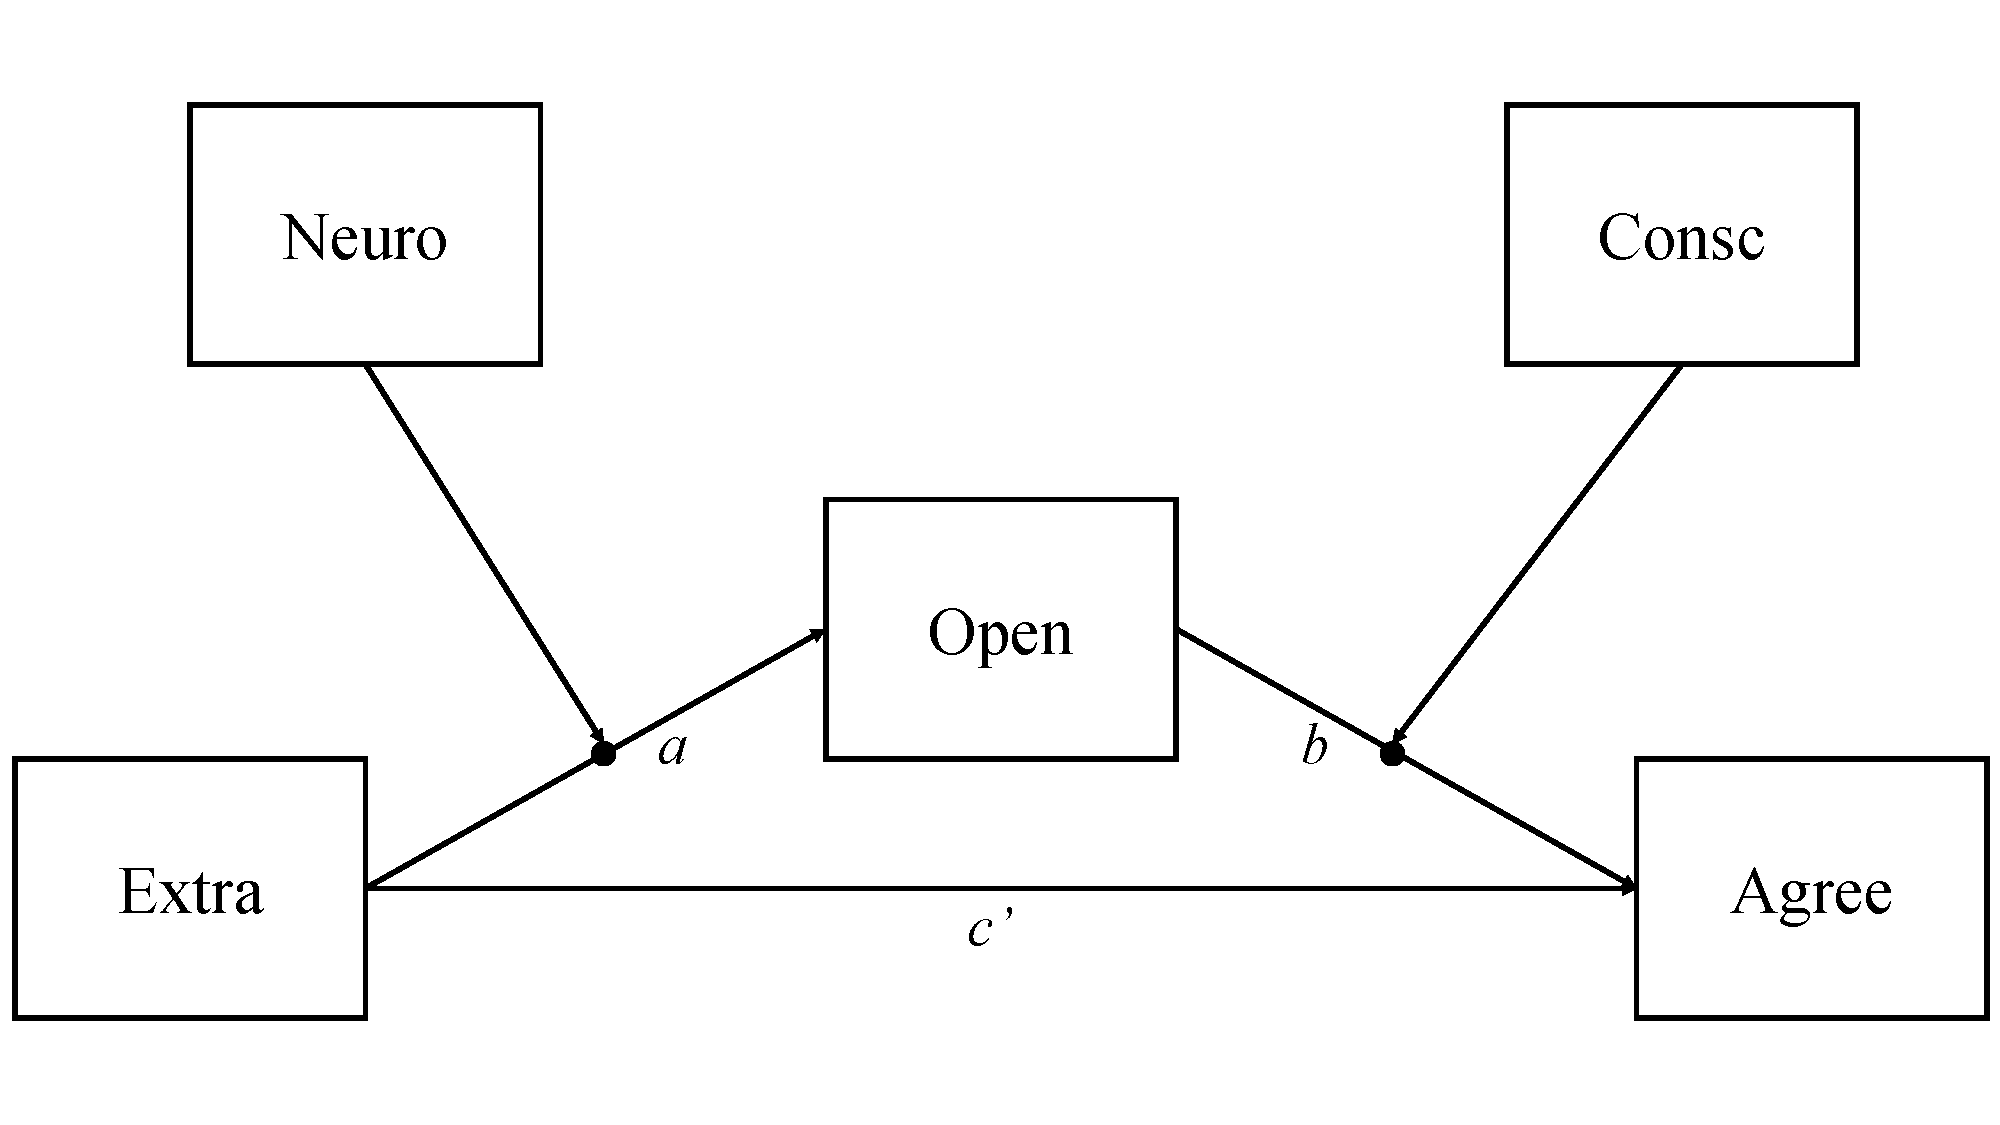
\includegraphics[width=0.95\textwidth]{figures/example3Conceptual.pdf}
  \end{figure}
  
\end{frame}



\begin{frame}{Example}
  
  The preceding conceptual model translates into the following
  analytic model: 
  \vb
  \begin{figure}
    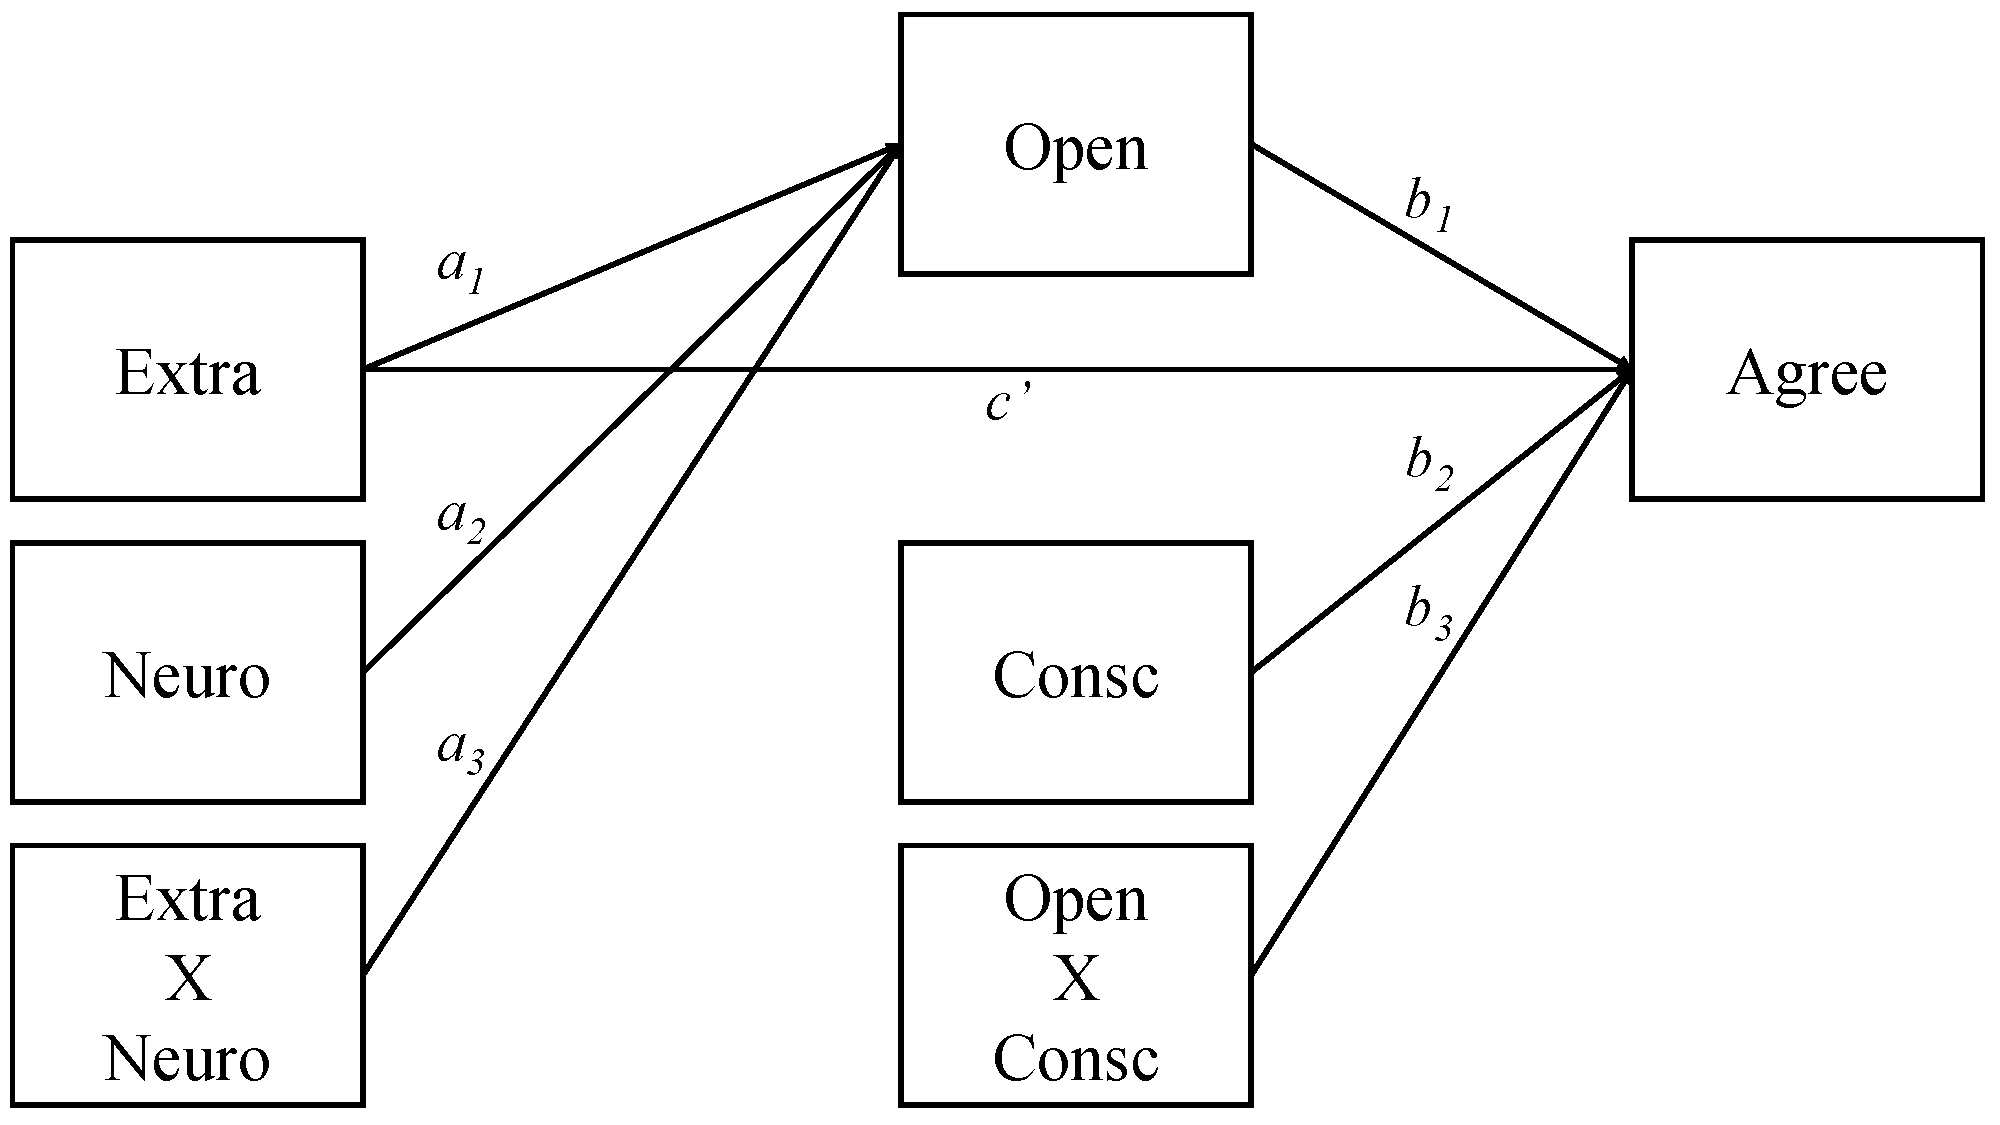
\includegraphics[width=0.95\textwidth]{figures/example3Analytic.pdf}
  \end{figure}
  
\end{frame}




\begin{frame}[shrink = 5]{Example}

\begin{Schunk}
\begin{Sinput}
 ## Completely Standardized:
 abCS <- (sdX * ab) / sdY
 abCS
\end{Sinput}
\begin{Soutput}
[1] 0.1345859
\end{Soutput}
\begin{Sinput}
 cPrimeCS <- (sdX * cPrime) / sdY
 cPrimeCS
\end{Sinput}
\begin{Soutput}
       cp 
0.1790413 
\end{Soutput}
\begin{Sinput}
 cCS <- abCS + cPrimeCS
 cCS
\end{Sinput}
\begin{Soutput}
       cp 
0.3136272 
\end{Soutput}
\end{Schunk}


\end{frame}



\begin{frame}[allowframebreaks]{Example}

\begin{Schunk}
\begin{Sinput}
 mod3 <- "
 fX =~ x1 + x2 + x3
 fZ =~ z1 + z2 + z3
 fY =~ y1 + y2 + y3
 fXZ =~ x1z1R + x1z2R + x1z3R +
 x2z1R + x2z2R + x2z3R +
 x3z1R + x3z2R + x3z3R
 
 fY ~ fX + fZ + fXZ
 
 fX ~~ fZ
 fX ~~ 0*fXZ
 fZ ~~ 0*fXZ
 
 x1z1R ~~ x1z2R + x1z3R + x2z1R + x3z1R
 x1z2R ~~ x1z3R + x2z2R + x3z2R
 x1z3R ~~ x2z3R + x3z3R
 
 x2z1R ~~ x2z2R + x2z3R + x3z1R
 x2z2R ~~ x2z3R + x3z2R
 x2z3R ~~ x3z3R
 
 x3z1R ~~ x3z2R + x3z3R
 x3z2R ~~ x3z3R
 "
 out3 <- sem(mod3, data = dat2, std.lv = TRUE)
 summary(out3)
\end{Sinput}
\begin{Soutput}
lavaan (0.5-20) converged normally after  53 iterations

  Number of observations                           500

  Estimator                                         ML
  Minimum Function Test Statistic               74.899
  Degrees of freedom                               113
  P-value (Chi-square)                           0.998

Parameter Estimates:

  Information                                 Expected
  Standard Errors                             Standard

Latent Variables:
                   Estimate  Std.Err  Z-value  P(>|z|)
  fX =~                                               
    x1                0.670    0.043   15.424    0.000
    x2                0.660    0.043   15.256    0.000
    x3                0.704    0.045   15.569    0.000
  fZ =~                                               
    z1                0.738    0.048   15.342    0.000
    z2                0.734    0.048   15.156    0.000
    z3                0.718    0.046   15.602    0.000
  fY =~                                               
    y1                0.396    0.046    8.545    0.000
    y2                0.369    0.044    8.441    0.000
    y3                0.383    0.045    8.558    0.000
  fXZ =~                                              
    x1z1R             0.361    0.053    6.833    0.000
    x1z2R             0.427    0.056    7.615    0.000
    x1z3R             0.432    0.053    8.190    0.000
    x2z1R             0.558    0.056    9.914    0.000
    x2z2R             0.616    0.062   10.008    0.000
    x2z3R             0.520    0.057    9.153    0.000
    x3z1R             0.516    0.059    8.805    0.000
    x3z2R             0.626    0.063   10.007    0.000
    x3z3R             0.521    0.058    8.936    0.000

Regressions:
                   Estimate  Std.Err  Z-value  P(>|z|)
  fY ~                                                
    fX                1.658    0.239    6.930    0.000
    fZ               -0.074    0.099   -0.750    0.453
    fXZ               0.488    0.120    4.049    0.000

Covariances:
                   Estimate  Std.Err  Z-value  P(>|z|)
  fX ~~                                               
    fZ                0.232    0.058    3.987    0.000
    fXZ               0.000                           
  fZ ~~                                               
    fXZ               0.000                           
  x1z1R ~~                                            
    x1z2R             0.273    0.032    8.397    0.000
    x1z3R             0.309    0.033    9.358    0.000
    x2z1R             0.232    0.031    7.566    0.000
    x3z1R             0.235    0.032    7.376    0.000
  x1z2R ~~                                            
    x1z3R             0.231    0.032    7.243    0.000
    x2z2R             0.211    0.035    5.982    0.000
    x3z2R             0.250    0.041    6.163    0.000
  x1z3R ~~                                            
    x2z3R             0.213    0.030    7.010    0.000
    x3z3R             0.213    0.034    6.312    0.000
  x2z1R ~~                                            
    x2z2R             0.247    0.043    5.787    0.000
    x2z3R             0.252    0.040    6.368    0.000
    x3z1R             0.233    0.033    7.103    0.000
  x2z2R ~~                                            
    x2z3R             0.304    0.043    7.086    0.000
    x3z2R             0.199    0.040    5.018    0.000
  x2z3R ~~                                            
    x3z3R             0.139    0.030    4.570    0.000
  x3z1R ~~                                            
    x3z2R             0.212    0.041    5.116    0.000
    x3z3R             0.260    0.040    6.454    0.000
  x3z2R ~~                                            
    x3z3R             0.157    0.041    3.846    0.000

Variances:
                   Estimate  Std.Err  Z-value  P(>|z|)
    x1                0.511    0.042   12.093    0.000
    x2                0.514    0.042   12.221    0.000
    x3                0.548    0.046   11.977    0.000
    z1                0.523    0.052   10.142    0.000
    z2                0.546    0.052   10.444    0.000
    z3                0.461    0.048    9.704    0.000
    y1                0.495    0.043   11.398    0.000
    y2                0.542    0.044   12.334    0.000
    y3                0.444    0.040   11.179    0.000
    x1z1R             0.743    0.050   14.912    0.000
    x1z2R             0.754    0.055   13.682    0.000
    x1z3R             0.694    0.050   13.824    0.000
    x2z1R             0.641    0.057   11.332    0.000
    x2z2R             0.708    0.067   10.575    0.000
    x2z3R             0.671    0.056   12.009    0.000
    x3z1R             0.736    0.060   12.310    0.000
    x3z2R             0.724    0.070   10.277    0.000
    x3z3R             0.707    0.060   11.823    0.000
    fX                1.000                           
    fZ                1.000                           
    fY                1.000                           
    fXZ               1.000                           
\end{Soutput}
\end{Schunk}


\pagebreak

\begin{Schunk}
\begin{Sinput}
 parameterEstimates(out2.1, boot = bootType)[ , -c(1 : 3)]
\end{Sinput}
\begin{Soutput}
     label    est    se      z pvalue ci.lower ci.upper
1       b1 -0.008 0.145 -0.052  0.959   -0.286    0.275
2       b2  0.595 0.142  4.184  0.000    0.317    0.861
3       cp  0.134 0.076  1.763  0.078   -0.019    0.281
4      d21 -0.301 0.110 -2.733  0.006   -0.508   -0.076
5       a2  0.090 0.072  1.253  0.210   -0.073    0.220
6       a1 -0.266 0.061 -4.384  0.000   -0.384   -0.148
7           0.987 0.164  6.013  0.000    0.733    1.390
8           0.689 0.094  7.309  0.000    0.537    0.919
9           0.719 0.112  6.389  0.000    0.535    0.980
10          2.444 0.000     NA     NA    2.444    2.444
11     ab1  0.002 0.040  0.050  0.960   -0.080    0.081
12     ab2  0.053 0.044  1.215  0.225   -0.031    0.146
13  fullIE  0.048 0.026  1.822  0.068    0.012    0.117
14 totalIE  0.103 0.048  2.145  0.032    0.011    0.202
\end{Soutput}
\end{Schunk}


\end{frame}




\begin{frame}{Example}
  
  Finally, maybe we think that \emph{neuroticism} also moderates the
  direct effect of \emph{extroversion} on \emph{agreeableness} (i.e.,
  the $c'$ path).\\ 
  \va 
  We can assess this conditional process via the following model:\\ 
  \vb
  \begin{figure}
    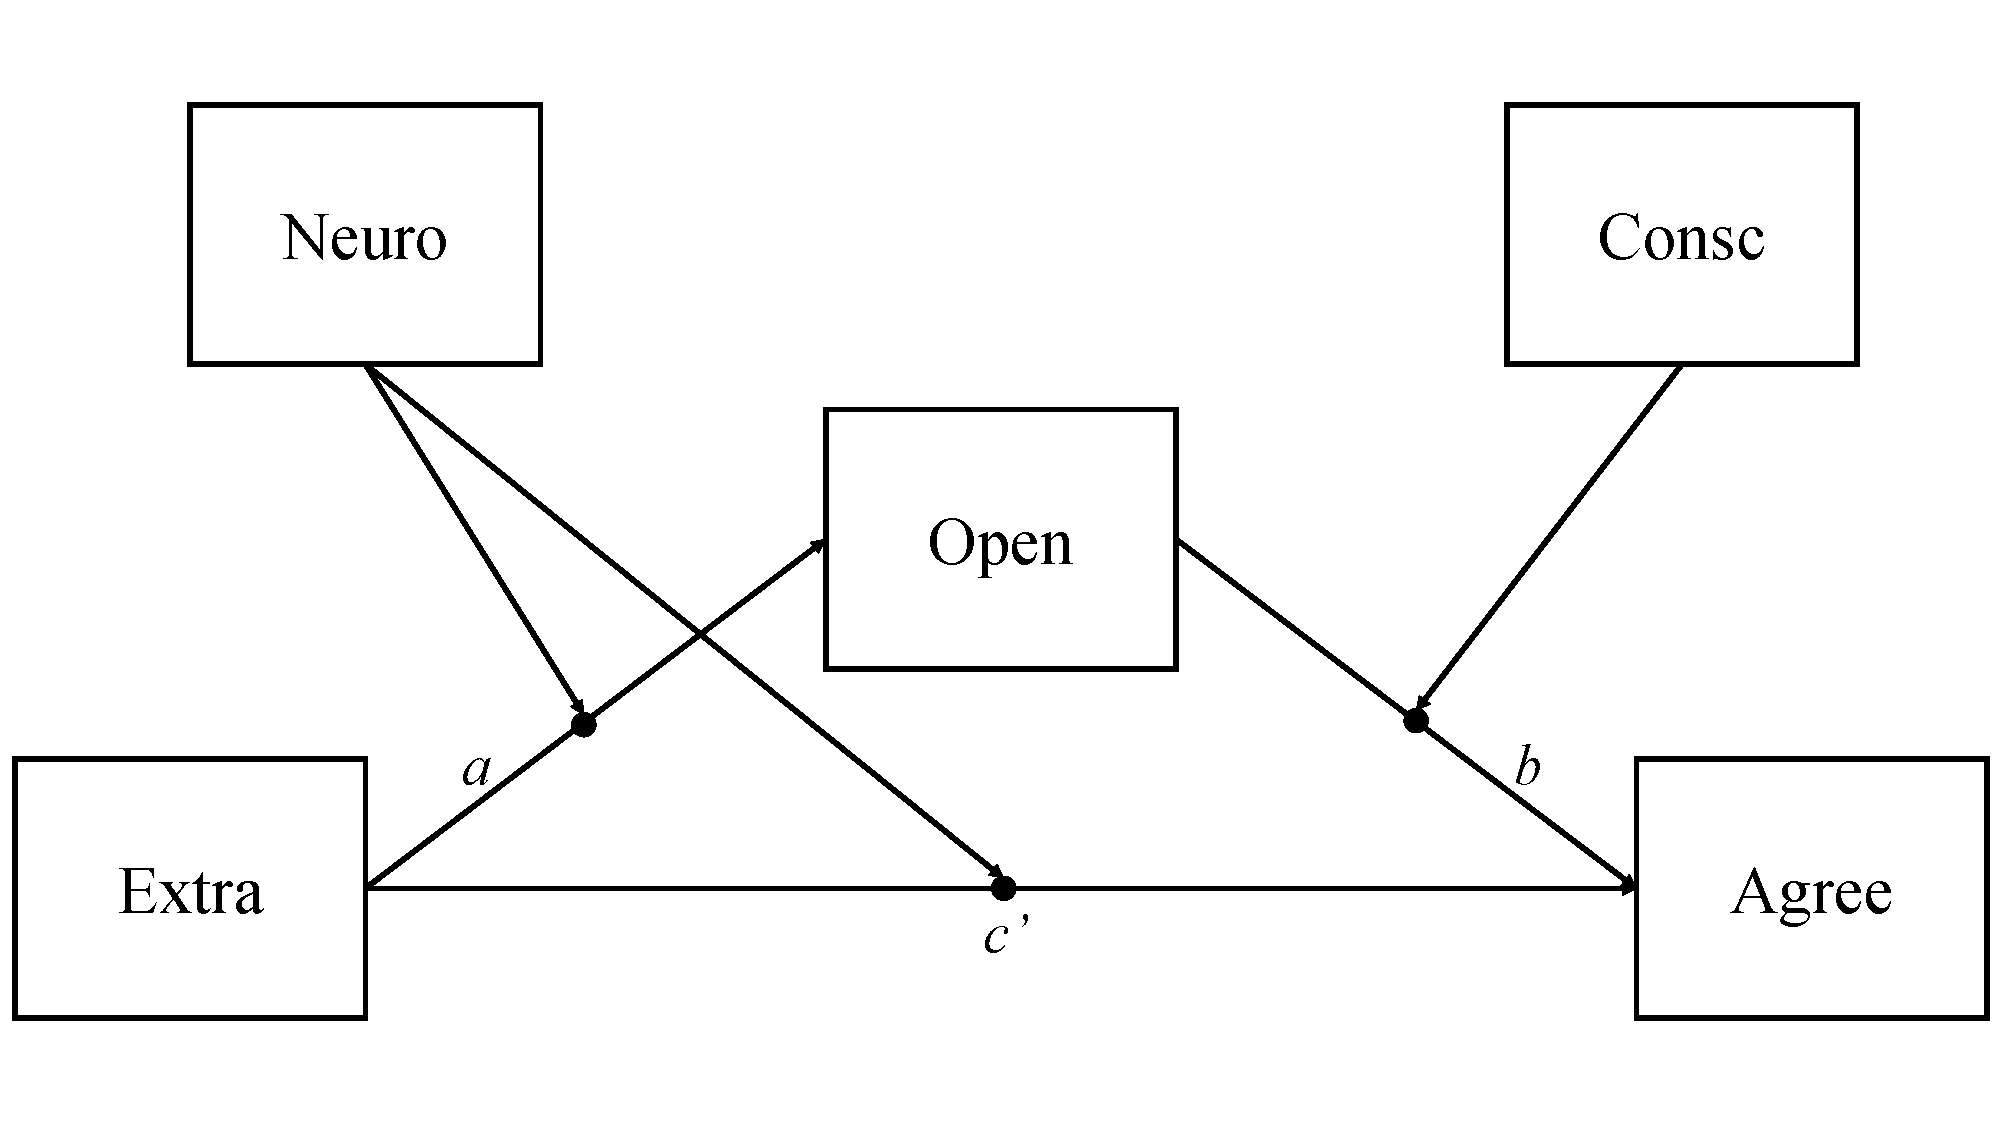
\includegraphics[width=0.95\textwidth]{figures/example4Conceptual.pdf}
  \end{figure}
  
\end{frame}




\begin{frame}{Example}
  
  The preceding conceptual model translates into the following
  analytic model: 
  \vb
  \begin{figure}
    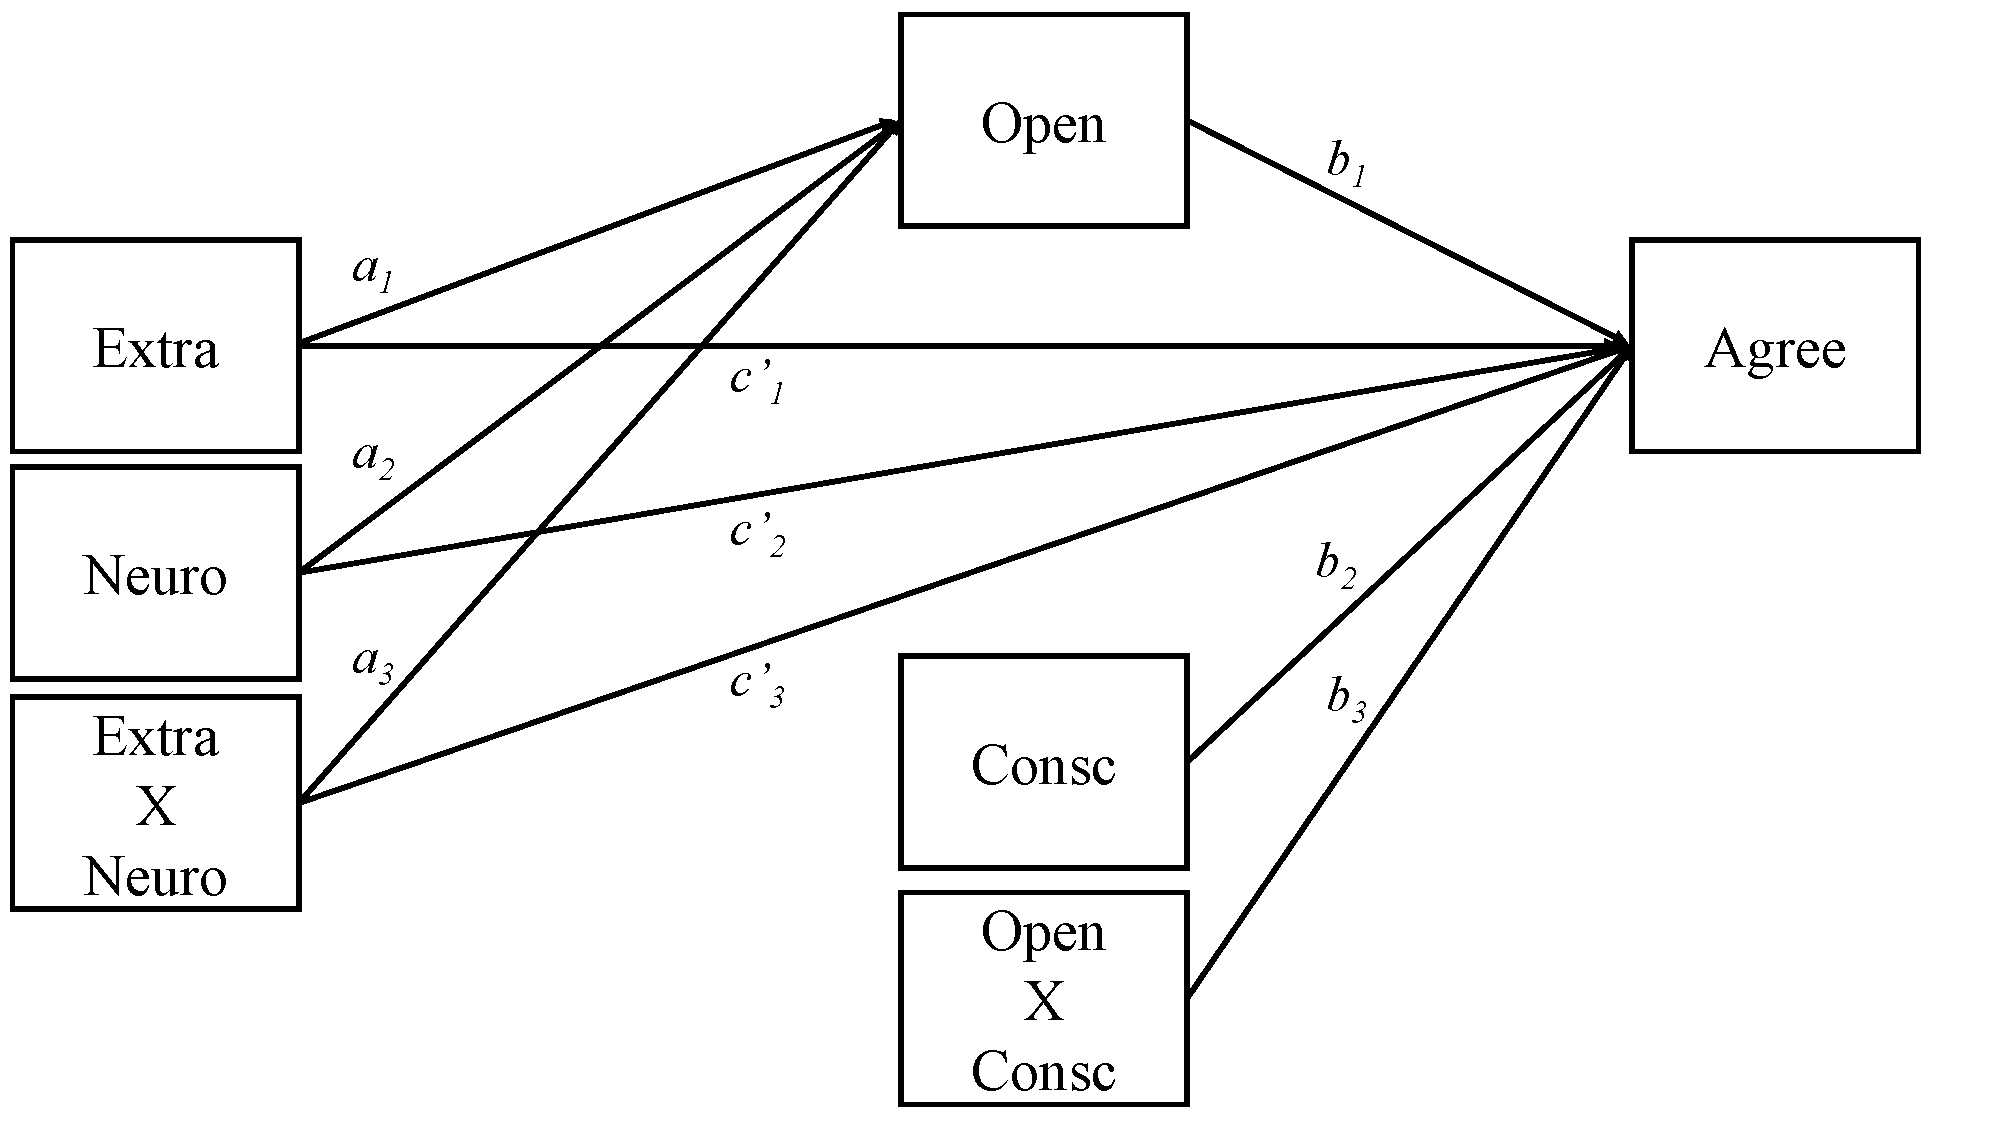
\includegraphics[width=0.95\textwidth]{figures/example4Analytic.pdf}
  \end{figure}
  
\end{frame}




\begin{frame}[allowframebreaks]{Example}

\begin{Schunk}
\begin{Sinput}
 ## Possible range of a:
 aMarg <- sqrt(s2M * s2Y - sYM^2) * sqrt(s2X * s2Y - sYX^2)
 aInt <- c(
     (sYM * sYX - aMarg) / (s2X * s2Y),
     (sYM * sYX + aMarg) / (s2X * s2Y)
 )
 aInt
\end{Sinput}
\begin{Soutput}
[1] -0.4378558  0.5793099
\end{Soutput}
\begin{Sinput}
 ##
 ## Possible range of b:
 bMarg <- sqrt(s2X * s2Y - sYX^2) / sqrt(s2X * s2M - sMX^2)
 bInt <- c(-1 * bMarg, bMarg)
 bInt
\end{Sinput}
\begin{Soutput}
[1] -1.289996  1.289996
\end{Soutput}
\begin{Sinput}
 ##
 ## max(a):
 aMax <- ifelse(coef(out2)["a"] < 0,
                aInt[1],
                aInt[2])
 aMax
\end{Sinput}
\begin{Soutput}
        a 
0.5793099 
\end{Soutput}
\begin{Sinput}
 ##
 ## max(b)
 bMax <- ifelse(coef(out2)["b"] < 0,
                bInt[1],
                bInt[2])
 bMax
\end{Sinput}
\begin{Soutput}
       b 
1.289996 
\end{Soutput}
\begin{Sinput}
 ##
 ## max(ab)
 abMax <- aMax * bMax
 abMax
\end{Sinput}
\begin{Soutput}
        a 
0.7473075 
\end{Soutput}
\begin{Sinput}
 ##
 ## Kappa Squared:
 k2 <- ab / abMax
 k2
\end{Sinput}
\begin{Soutput}
        a 
0.1359491 
\end{Soutput}
\end{Schunk}


\pagebreak

\begin{Schunk}
\begin{Sinput}
 ## Three-way interaction model:
 out1.3 <- lm(agree ~ open*conc*neuro, data = dat1)
 summary(out1.3)
\end{Sinput}
\begin{Soutput}
Call:
lm(formula = agree ~ open * conc * neuro, data = dat1)

Residuals:
     Min       1Q   Median       3Q      Max 
-2.79789 -0.41779  0.09925  0.47556  2.10928 

Coefficients:
                Estimate Std. Error t value Pr(>|t|)    
(Intercept)     -0.58747    0.96633  -0.608  0.54328    
open             1.27903    0.25747   4.968 7.23e-07 ***
conc             1.20831    0.26559   4.550 5.63e-06 ***
neuro            0.73766    0.32240   2.288  0.02222 *  
open:conc       -0.29722    0.06935  -4.286 1.89e-05 ***
open:neuro      -0.21616    0.08091  -2.672  0.00760 ** 
conc:neuro      -0.25632    0.08244  -3.109  0.00190 ** 
open:conc:neuro  0.06541    0.02028   3.225  0.00128 ** 
---
Signif. codes:  0 ‘***’ 0.001 ‘**’ 0.01 ‘*’ 0.05 ‘.’ 0.1 ‘ ’ 1

Residual standard error: 0.6945 on 2544 degrees of freedom
Multiple R-squared:  0.07189,	Adjusted R-squared:  0.06933 
F-statistic: 28.15 on 7 and 2544 DF,  p-value: < 2.2e-16
\end{Soutput}
\end{Schunk}


\pagebreak

\begin{Schunk}
\begin{Sinput}
 ## Test Differences between Indirect Effects
 ## in Serial Multiple Mediator Model (Method 1):
 mod2.3 <- "
 policy ~ cp*polAffil + b1*merit + b2*sysRac
 merit ~ a1*polAffil
 sysRac ~ a2*polAffil + d21*merit
 
 ab1 := a1*b1
 ab2 := a2*b2
 fullIE := a1*d21*b2
 totalIE := ab1 + ab2 + fullIE 
 
 fullIE == ab1
 fullIE == ab2
 "
 out2.3 <- 
     sem(mod2.3, data = dat1, se = "boot", boot = nBoot)
 summary(out2.3)
\end{Sinput}
\begin{Soutput}
lavaan (0.5-20) converged normally after 213 iterations

  Number of observations                            87

  Estimator                                         ML
  Minimum Function Test Statistic                1.334
  Degrees of freedom                                 2
  P-value (Chi-square)                           0.513

Parameter Estimates:

  Information                                 Observed
  Standard Errors                            Bootstrap
  Number of requested bootstrap draws             2500
  Number of successful bootstrap draws            2500

Regressions:
                   Estimate  Std.Err  Z-value  P(>|z|)
  policy ~                                            
    polAffil  (cp)    0.108    0.084    1.281    0.200
    merit     (b1)   -0.150    0.047   -3.183    0.001
    sysRac    (b2)    0.521    0.125    4.157    0.000
  merit ~                                             
    polAffil  (a1)   -0.271    0.057   -4.750    0.000
  sysRac ~                                            
    polAffil  (a2)    0.078    0.025    3.125    0.002
    merit    (d21)   -0.287    0.075   -3.814    0.000

Variances:
                   Estimate  Std.Err  Z-value  P(>|z|)
    policy            1.001    0.171    5.854    0.000
    merit             0.719    0.114    6.330    0.000
    sysRac            0.690    0.090    7.632    0.000

Defined Parameters:
                   Estimate  Std.Err  Z-value  P(>|z|)
    ab1               0.041    0.014    2.983    0.003
    ab2               0.041    0.014    2.983    0.003
    fullIE            0.041    0.014    2.983    0.003
    totalIE           0.122    0.041    2.983    0.003

Constraints:
                                               |Slack|
    fullIE - (ab1)                               0.000
    fullIE - (ab2)                               0.000
\end{Soutput}
\begin{Sinput}
 ## Conduct a chi-squared difference test:
 chiDiff <- fitMeasures(out2.3)["chisq"] - 
     fitMeasures(out2.1)["chisq"]
 dfDiff <- fitMeasures(out2.3)["df"] - 
     fitMeasures(out2.1)["df"]
 pchisq(chiDiff, dfDiff, lower = FALSE)
\end{Sinput}
\begin{Soutput}
    chisq 
0.5131246 
\end{Soutput}
\end{Schunk}


\end{frame}



\begin{frame}[allowframebreaks]{Example}

  The $a$ path was not significantly moderated in any of the previous
  models.
  \begin{itemize}
    \item Maybe we should try culling that path to see if we can get a
      more parsimonious description of the process.  
  \end{itemize}
  \va
\begin{Schunk}
\begin{Sinput}
 ## Conditional process model with b, c paths moderated:
 mod5 <- "
 agree ~ b1*open + b2*consc + cp1*extra + cp2*neuro + 
         cp3*extraXneuro + b3*openXconsc
 open ~ a*extra
 
 cpLo  := cp1 + cp3*(-0.962268)
 cpMid := cp1 + cp3*(-0.162268)
 cpHi  := cp1 + cp3*0.837732
 
 abLo := a * (b1 + b3*(-0.4045))
 abMid := a * (b1 + b3*(-0.0045))
 abHi := a * (b1 + b3*0.3955)
 "
\end{Sinput}
\end{Schunk}


\pagebreak

\begin{Schunk}
\begin{Sinput}
 out5 <- sem(mod5, data = dat1, se = "boot", boot = nBoot)
 summary(out5)
\end{Sinput}
\begin{Soutput}
lavaan (0.5-20) converged normally after  18 iterations

  Number of observations                          2800

  Estimator                                         ML
  Minimum Function Test Statistic              201.443
  Degrees of freedom                                 4
  P-value (Chi-square)                           0.000

Parameter Estimates:

  Information                                 Observed
  Standard Errors                            Bootstrap
  Number of requested bootstrap draws             5000
  Number of successful bootstrap draws            5000

Regressions:
                   Estimate  Std.Err  Z-value  P(>|z|)
  agree ~                                             
    open      (b1)    0.191    0.028    6.941    0.000
    consc     (b2)    0.021    0.027    0.774    0.439
    extra    (cp1)    0.349    0.027   13.030    0.000
    neuro    (cp2)   -0.102    0.012   -8.564    0.000
    extraXnr (cp3)    0.049    0.022    2.210    0.027
    opnXcnsc  (b3)   -0.074    0.044   -1.671    0.095
  open ~                                              
    extra      (a)    0.268    0.023   11.662    0.000

Variances:
                   Estimate  Std.Err  Z-value  P(>|z|)
    agree             0.471    0.014   32.521    0.000
    open              0.294    0.010   29.875    0.000

Defined Parameters:
                   Estimate  Std.Err  Z-value  P(>|z|)
    cpLo              0.302    0.036    8.459    0.000
    cpMid             0.341    0.027   12.473    0.000
    cpHi              0.390    0.031   12.502    0.000
    abLo              0.059    0.011    5.320    0.000
    abMid             0.051    0.009    5.778    0.000
    abHi              0.043    0.009    4.788    0.000
\end{Soutput}
\end{Schunk}


\pagebreak

\begin{Schunk}
\begin{Sinput}
 ## Hybrid Multiple Mediator Model:
 mod4.1 <- "
 policy ~ b1*merit + b21*sysRac + b22*revDisc + cp*polAffil
 sysRac ~ d211*merit + a21*polAffil
 revDisc ~ d221*merit + a22*polAffil
 merit ~ a1*polAffil
 
 sysRac ~~ revDisc
 
 ab1 := a1*b1
 ab21 := a21*b21
 ab22 := a22*b22
 
 fullIE21 := a1*d211*b21
 fullIE22 := a1*d221*b22
 
 totalIE := ab1 + ab21 + ab22 + fullIE21 + fullIE22
 "
 out4.1 <- 
     sem(mod4.1, data = dat1, se = "boot", boot = nBoot)
 summary(out4.1)
\end{Sinput}
\begin{Soutput}
lavaan (0.5-20) converged normally after  22 iterations

  Number of observations                            87

  Estimator                                         ML
  Minimum Function Test Statistic                0.000
  Degrees of freedom                                 0
  Minimum Function Value               0.0000000000000

Parameter Estimates:

  Information                                 Observed
  Standard Errors                            Bootstrap
  Number of requested bootstrap draws             2500
  Number of successful bootstrap draws            2499

Regressions:
                   Estimate  Std.Err  Z-value  P(>|z|)
  policy ~                                            
    merit     (b1)    0.005    0.142    0.035    0.972
    sysRac   (b21)    0.589    0.150    3.924    0.000
    revDisc  (b22)   -0.026    0.080   -0.328    0.743
    polAffl   (cp)    0.130    0.080    1.627    0.104
  sysRac ~                                            
    merit   (d211)   -0.301    0.111   -2.721    0.006
    polAffl  (a21)    0.090    0.070    1.282    0.200
  revDisc ~                                           
    merit   (d221)    0.532    0.192    2.777    0.005
    polAffl  (a22)   -0.167    0.138   -1.214    0.225
  merit ~                                             
    polAffl   (a1)   -0.266    0.061   -4.337    0.000

Covariances:
                   Estimate  Std.Err  Z-value  P(>|z|)
  sysRac ~~                                           
    revDisc          -0.135    0.157   -0.859    0.390

Variances:
                   Estimate  Std.Err  Z-value  P(>|z|)
    policy            0.985    0.162    6.098    0.000
    sysRac            0.689    0.092    7.463    0.000
    revDisc           2.388    0.303    7.881    0.000
    merit             0.719    0.113    6.378    0.000

Defined Parameters:
                   Estimate  Std.Err  Z-value  P(>|z|)
    ab1              -0.001    0.039   -0.034    0.973
    ab21              0.053    0.043    1.247    0.212
    ab22              0.004    0.018    0.251    0.801
    fullIE21          0.047    0.025    1.871    0.061
    fullIE22          0.004    0.014    0.276    0.783
    totalIE           0.107    0.052    2.047    0.041
\end{Soutput}
\end{Schunk}


\end{frame}


\end{document}
